\documentclass[12pt,a4paper]{report}
\usepackage[pdftex]{graphicx}
\usepackage{url} 
\usepackage{svg}
\usepackage{multicol}
\usepackage{booktabs}
\usepackage{graphicx}
\usepackage{gensymb}
\usepackage{enumitem}
\usepackage{placeins}
    \setlist[itemize]{itemsep=0mm}
\usepackage[utf8]{inputenc}
\usepackage[english]{babel}
\usepackage{chemfig}
    \setchemfig{
        atom sep        = 2em,
        bond join       = true,
    }
\usepackage{chemmacros}
    \chemsetup{
        modules = {all},
    }
\usepackage[bookmarks, colorlinks=false, pdfborder={0 0 0}, pdftitle={<pdf title here>}, pdfauthor={<author's name here>}, pdfsubject={<subject here>}, pdfkeywords={<keywords here>}]{hyperref} 

\newcommand{\email}[1]{{\tt#1}}
\newcommand{\udl}[1]{{\underline{#1}}}
\newcommand{\bd}[1]{{\textbf{#1}}}



\begin{document}


\begin{titlepage}
\normalsize \text{University of Cambridge Engineering Tripos Part IIA 2020/21}\\[2in]
\begin{center}

\LARGE \textbf {3G1: Molecular Bioengineering I \\[.1in] Lecture Notes}\\[3in]


       

% Submitted by
\normalsize \textbf{Connor Wang}\\[.2in]
\email{xw345@cam.ac.uk}\\
Engineering Undergraduate\\
Magdalene College, University of Cambridge\\


\end{center}

\end{titlepage}

\vspace{2in}
\begin{abstract}
\vspace{.4in}
The abstract of this course will be filled in when all the courses are delivered.

\end{abstract} 


\pagenumbering{roman}
\tableofcontents


\newpage
\pagenumbering{arabic} 

% \input{prob-definition} 
\chapter{Evolution I}

\section{Introduction to Evolution}

\begin{enumerate}
    \item All living organisms are related through the examination of their DNA sequences. Mass extinctions happened for several times.
    \item Evolution has given rise to huge \textit{diversity}. There are probably more than 10 million species.
    \item Evolution also operates on \textit{massive numbers} of individuals \textit{in parallel}.
\end{enumerate}



\section{Evolution at the molecular level}

\begin{enumerate}
    \item RNA may well have been the first self-replicating molecule to evolve. It is capable of more interesting chemistry and has \textit{lower stability} than DNA.
    \item The greater stability of DNA makes it more suitable for the storage and transmission of information between \textit{generations}.
\end{enumerate}



\section{Quiz 1: Combination of mutated genes}

\bd{Question set}\\[.1in]
An organism divides to make two daughters. Different granddaughters (red, blue) acquire different (rare) mutations that let them and their children grow faster. Perhaps the combination will be even better! Given the random nature of mutations it would take too long for the double mutant to arise by chance. Life has evolved to evolve quickly. What must be going on? Simple and complex organisms have different solutions. \\[.2in]
\bd{Answer}\\[.1in]
As shown, DNA is transferred vertically from parent to child. In order that the different mutations (red, blue) can be combined in one organism there must be some kind of \textit{horizontal transfer} of DNA sequences.
\begin{enumerate}
    \item \bd{Simple organism: Horizontal gene transfer}\\ In prokaryotes\footnote{Prokaryotes are unicellular organisms that lack organelles or other internal membrane-bound structures.}, such horizontal gene transfer is mediated by several mechanisms (conjugation\footnote{A specific mechanism to transfer DNA between cells. The basis for much antibiotic resistance, which can be transferred quite efficiently.}, transduction\footnote{Viruses pick up and move random host genes to new cells.}, transformation\footnote{Random uptake of DNA from the environment} or molecular bioenineering). These transfers tend to involve \udl{transfers} of short lengths of DNA (compared to the total length of the chromosome), and can be random and infrequent.
    
   \item \bd{Complex organism: Sexual reproduction}\\ In complex organisms, \udl{sexual reproduction} allows an extremely efficient mixing of DNA as each child receives a single complement of genetic information ($n$ chromosomes) from each parent ($2n$). Furthermore, the parental chromosome pairs line up and recombine before being passed on, so that a new combination of variations is passed on.
\end{enumerate}


\section{Evolutionary and phylogenetic trees}

\begin{enumerate}
    \item \bd{Prokaryotes} Prokaryotes have no membrane-surrounded nucleus containing DNA, as the eukaryotes do.
    \begin{enumerate}
        \item \bd{Archaea} Archaea include most of the extremophiles but also methane-generating gut bacteria.
        \item \bd{Bacteria}
    \end{enumerate}
    \item \bd{Eukaryotes} Eukaryotes have \udl{cells} with \udl{complex} internal structures and include all the Eukaryotes plants and animals but also microbes e.g. yeast\footnote{A type of fungus commonly used for alcoholic beverages and baking.}. The original eukaryotes are likely to have formed through a symbiosis between archeal and bacterial cells.
\end{enumerate}


\section{A View of Darwinian evolution}

\begin{figure}[h]
\centering
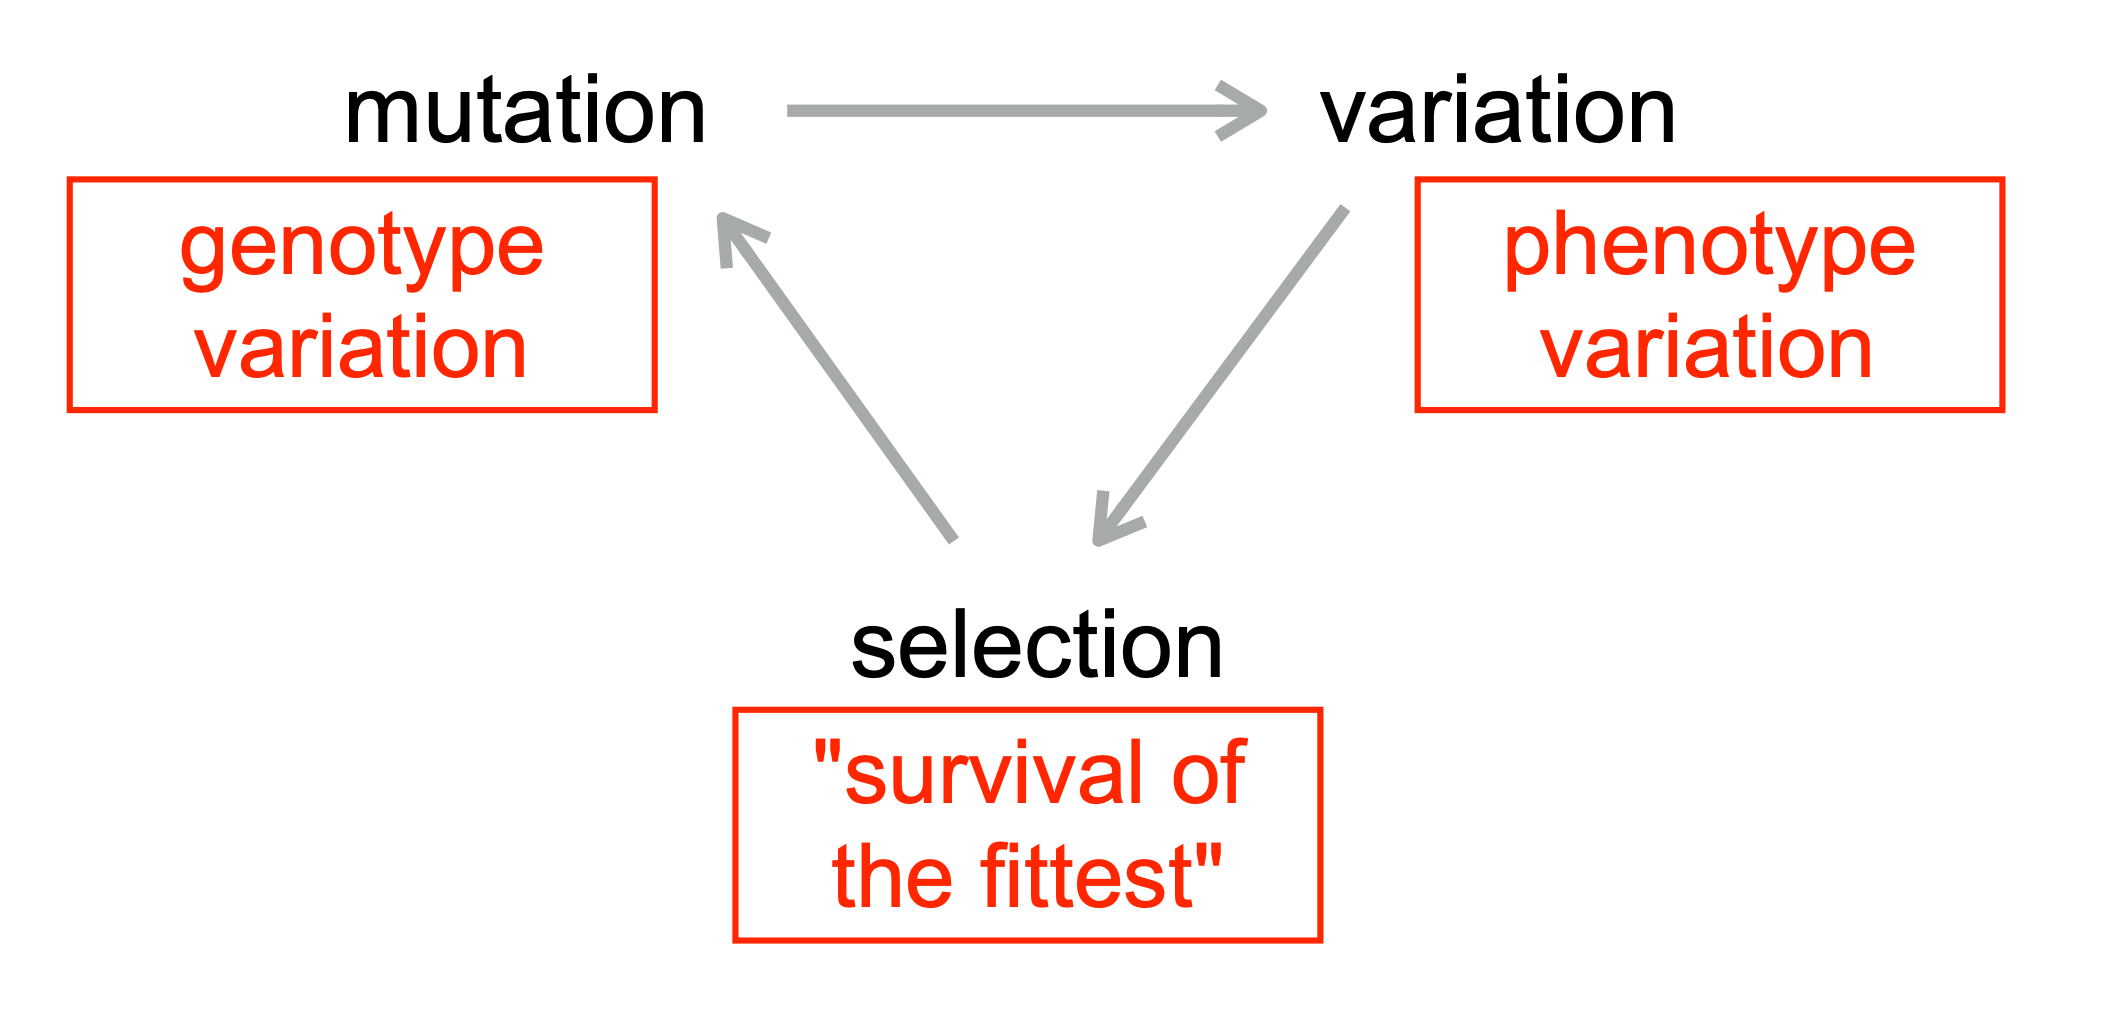
\includegraphics[width=1\textwidth]{images/lecture1.png}\\[.2in]
\caption{A View of Darwinian evolution} 
\end{figure}


\section{Quiz 2: Interfere evolution}
Given the Darwinian evolution graph, where can we interfere?
\begin{enumerate}
    \item \bd{mutation}: random mutagenesis, design specific mutations or introduce new functions.
    \item \bd{phenotypic variation}: conducive environment.
    \item \bd{selection}: artificial selection.
\end{enumerate} 
\chapter{Evolution II}

Key question: is evolution an experimentally testable theory?
\section{Case study: The Lenski Affair}

\begin{itemize}
    \item Starting at 1988, 12 identical cit- cultures (cit+ anaerobically) grew with limiting glucose and excess citrate.
    \item Dilute everyday and repeat freezing samples every 500 generations for about 30 years.
    \item In one culture only, weakly citrate-using (cit+) growth at generation about 31,500 is observed. And about 2000 more generations leads to strong cit+ growth.
    \item The experiment can be \textit{replayed} using the frozen samples.
\end{itemize}
This experiments provide evidence for potentiating mutation(s). It is an evolution under controlled laboratory conditions.

\section{Quiz 1: An always inherited gene}
\bd{Question} \\ [.1in]
How might we engineer an organism so that an altered gene (for flies) would always spread? \\ [.2in]
\bd{Solution} \\ [.1in]
Flies are complex organisms which \udl{reproduce sexually}. Each parent donates one chromosome from each of its pairs to the child. In this example the "red" gene is dominant in the sense that a single copy leads to the "red" phenotype.\\[.2in]
\bd{Normal inheritance}: the red fly has a "red" gene on one chromosome and a normal (blue) gene on the other as can be seen by the fact that it produces both red and blue children. If red flies always have to mate with blue flies, the red gene \udl{does not spread}.\\[.2in]
\bd{Gene drive inheritance}: the "red" gene \udl{drive gene copies} itself to the "blue" chromosome so that it is passed on to \textit{all} the children. This can be used in the lab to make mosquito populations sterile. This has not been tested in the wild, yet.
\begin{figure}[h]
\centering
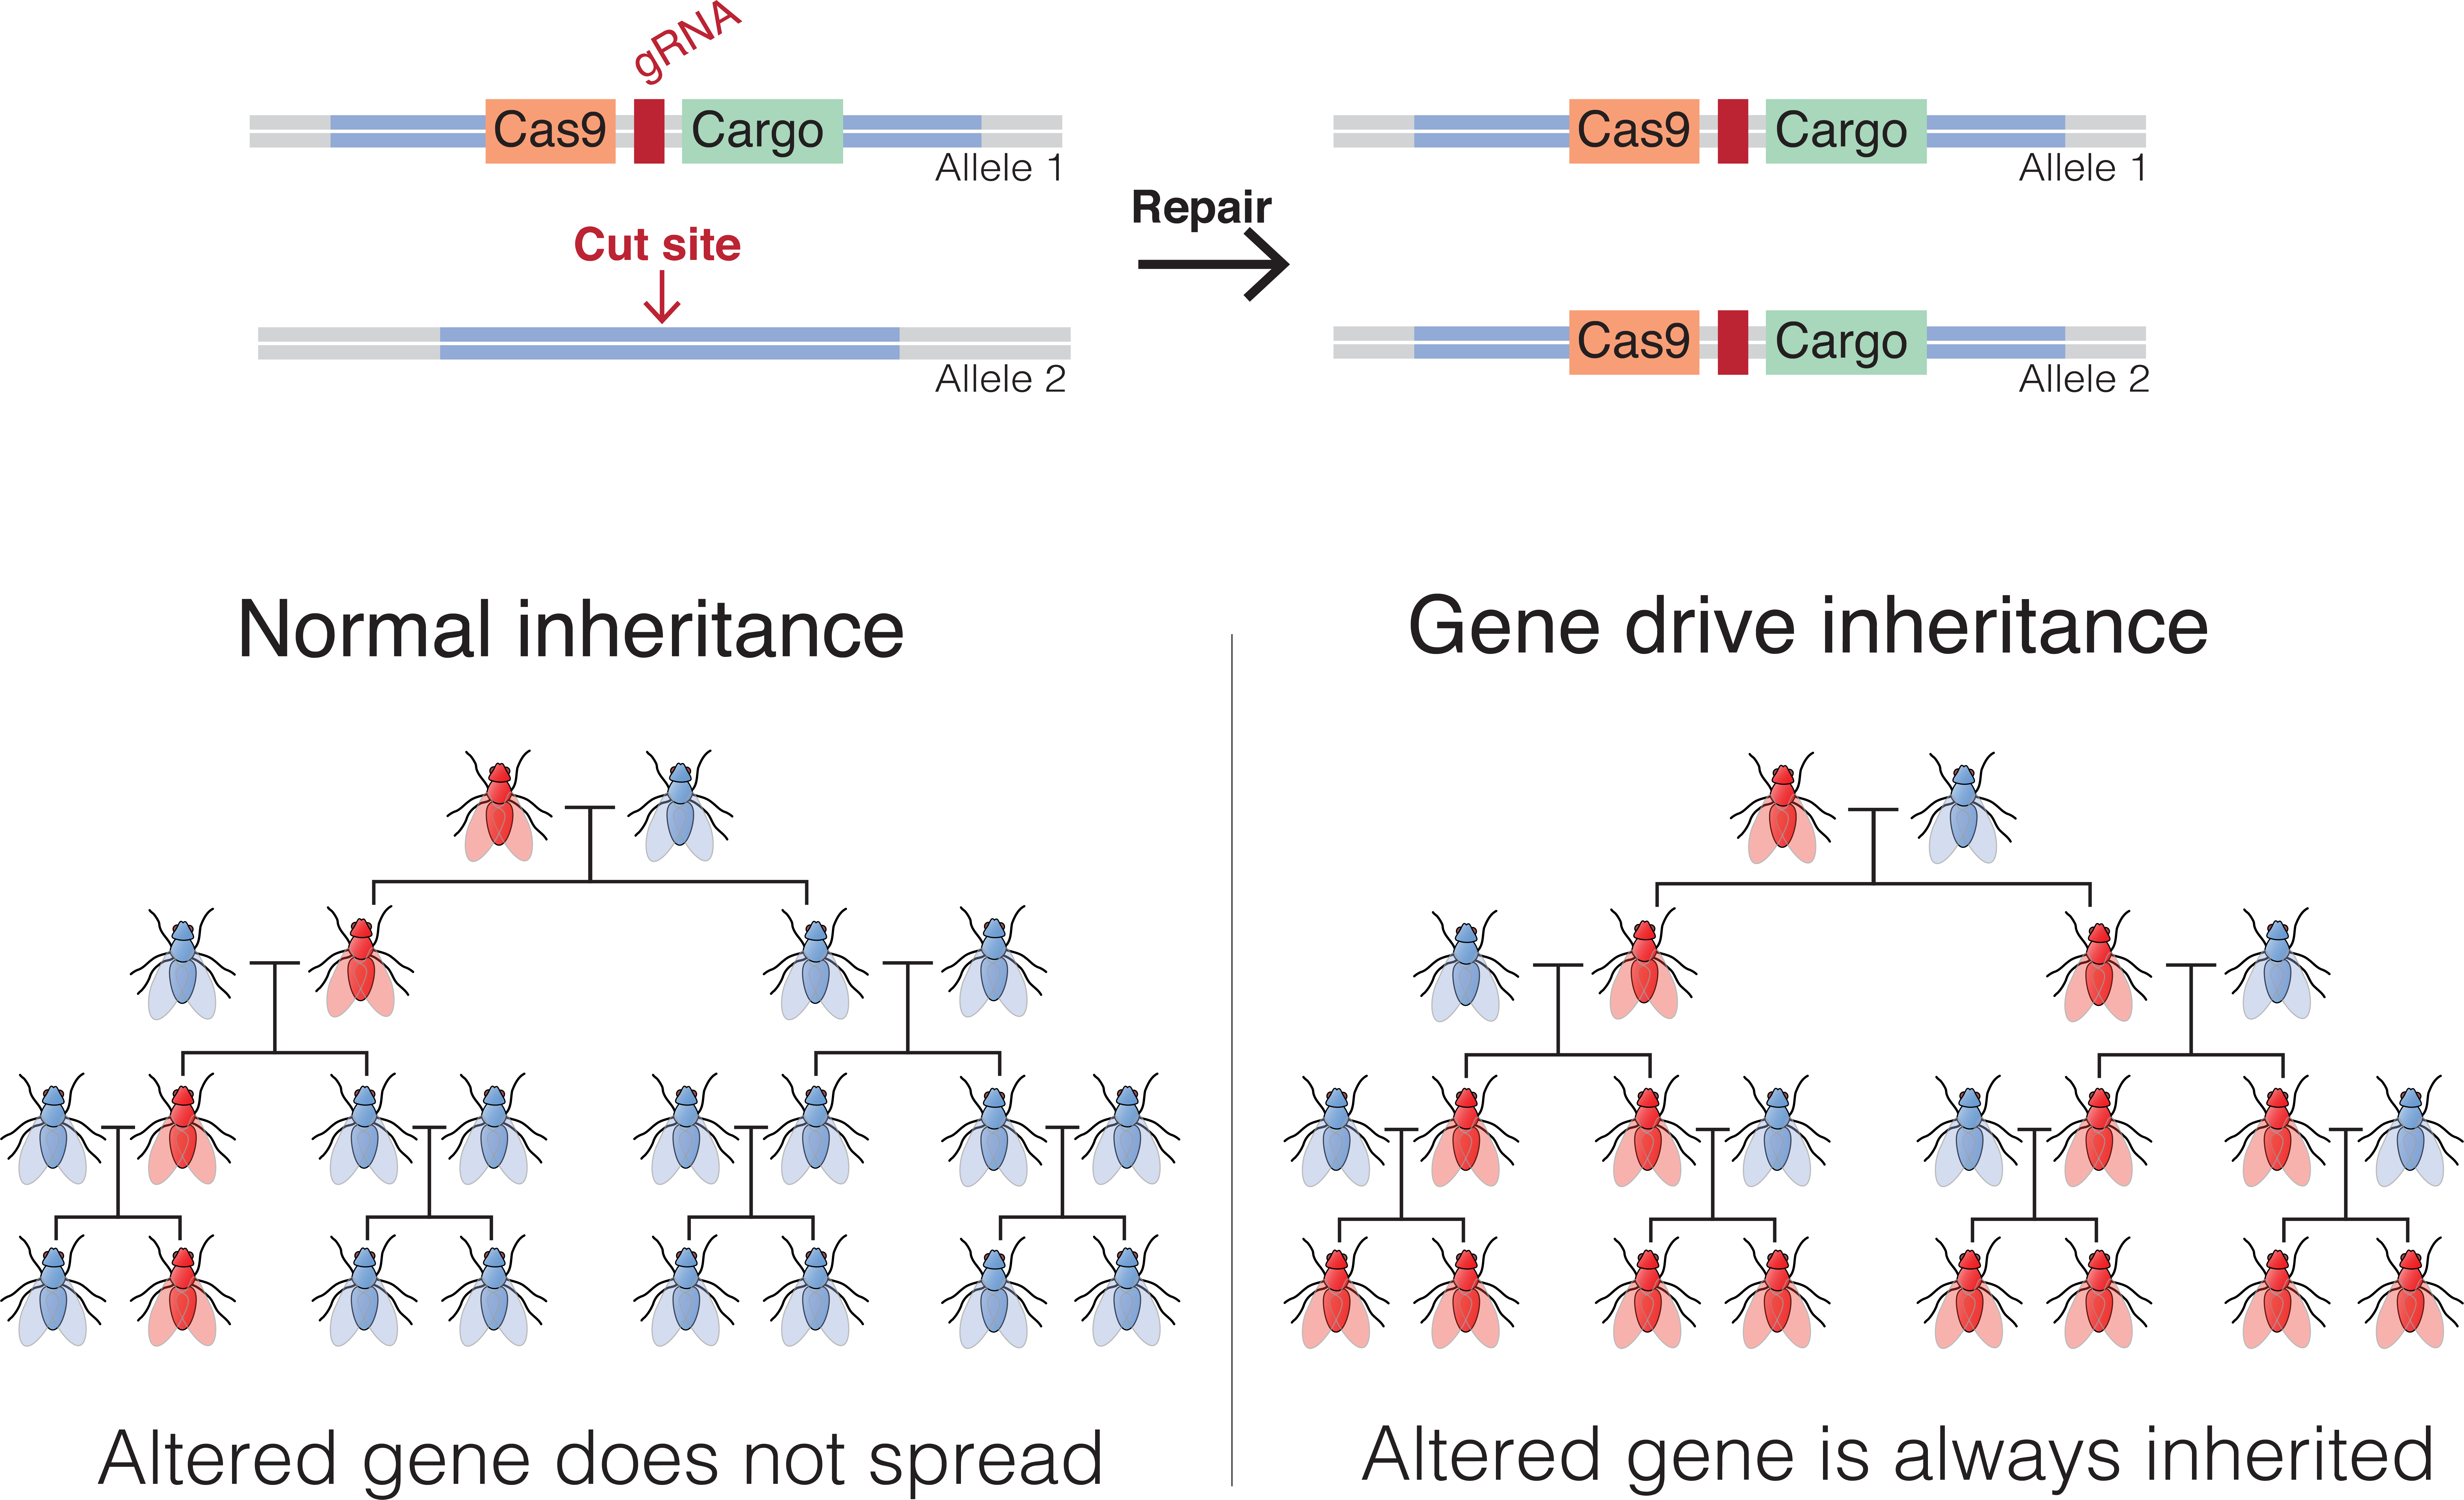
\includegraphics[width=1\textwidth]{images/Gene_Drive.png}\\[.2in]
\caption{Quiz 1 illustration} 
\end{figure}

\section{Innate and Adaptive immune systems}
Both prokaryotes and eukaryotes have \udl{innate} and \udl{adaptive} \textit{immune systems} to protect them. These systems have provided excellent tools to bioengineers.
\begin{enumerate}
    \item \bd{Prokarotes}
    \begin{enumerate}
        \item \bd{Innate: Restriction enzymes}\\ Proteins that cut DNA at specific sequence (evolved to protect against viruses)
        \item \bd{Adaptive: CRISPR/cas9}\\ Programmable cutting of DNA, and more (evolved to protect against viruses)
    \end{enumerate}
    \item \bd{Eukaryotes}
    \begin{enumerate}
        \item \bd{Innate:} no typical example
        \item \bd{Adaptive: Antibodies}\\ Proteins that can bind to other molecules tightly and with high specificity (evolved to recognise pathogens\footnote{A bacterium, virus, or other microorganism that can cause disease.} and recruit responder cells)

    \end{enumerate}
\end{enumerate}

\chapter{Central Dogma}

\section{Base Pairing and the Double Helix}
The chemical structure of each base allows it to match up with another.
\begin{itemize}
    \item Guanine - Cytosine (G - C): Three Hydrophone bond
    \item Adenine - Thymine (A - T): Two Hydrophone bond
    \item Start of the sequence: 5' end
    \item End of the sequence: 3' end
\end{itemize}

\section{Ribonucleic acid (RNA) and Deoxribonucleic acid (DNA)}

DNA and RNA are composed of similar monomer building blocks. They provides ultra high density base-4 memory.

\begin{figure}[h]
\centering
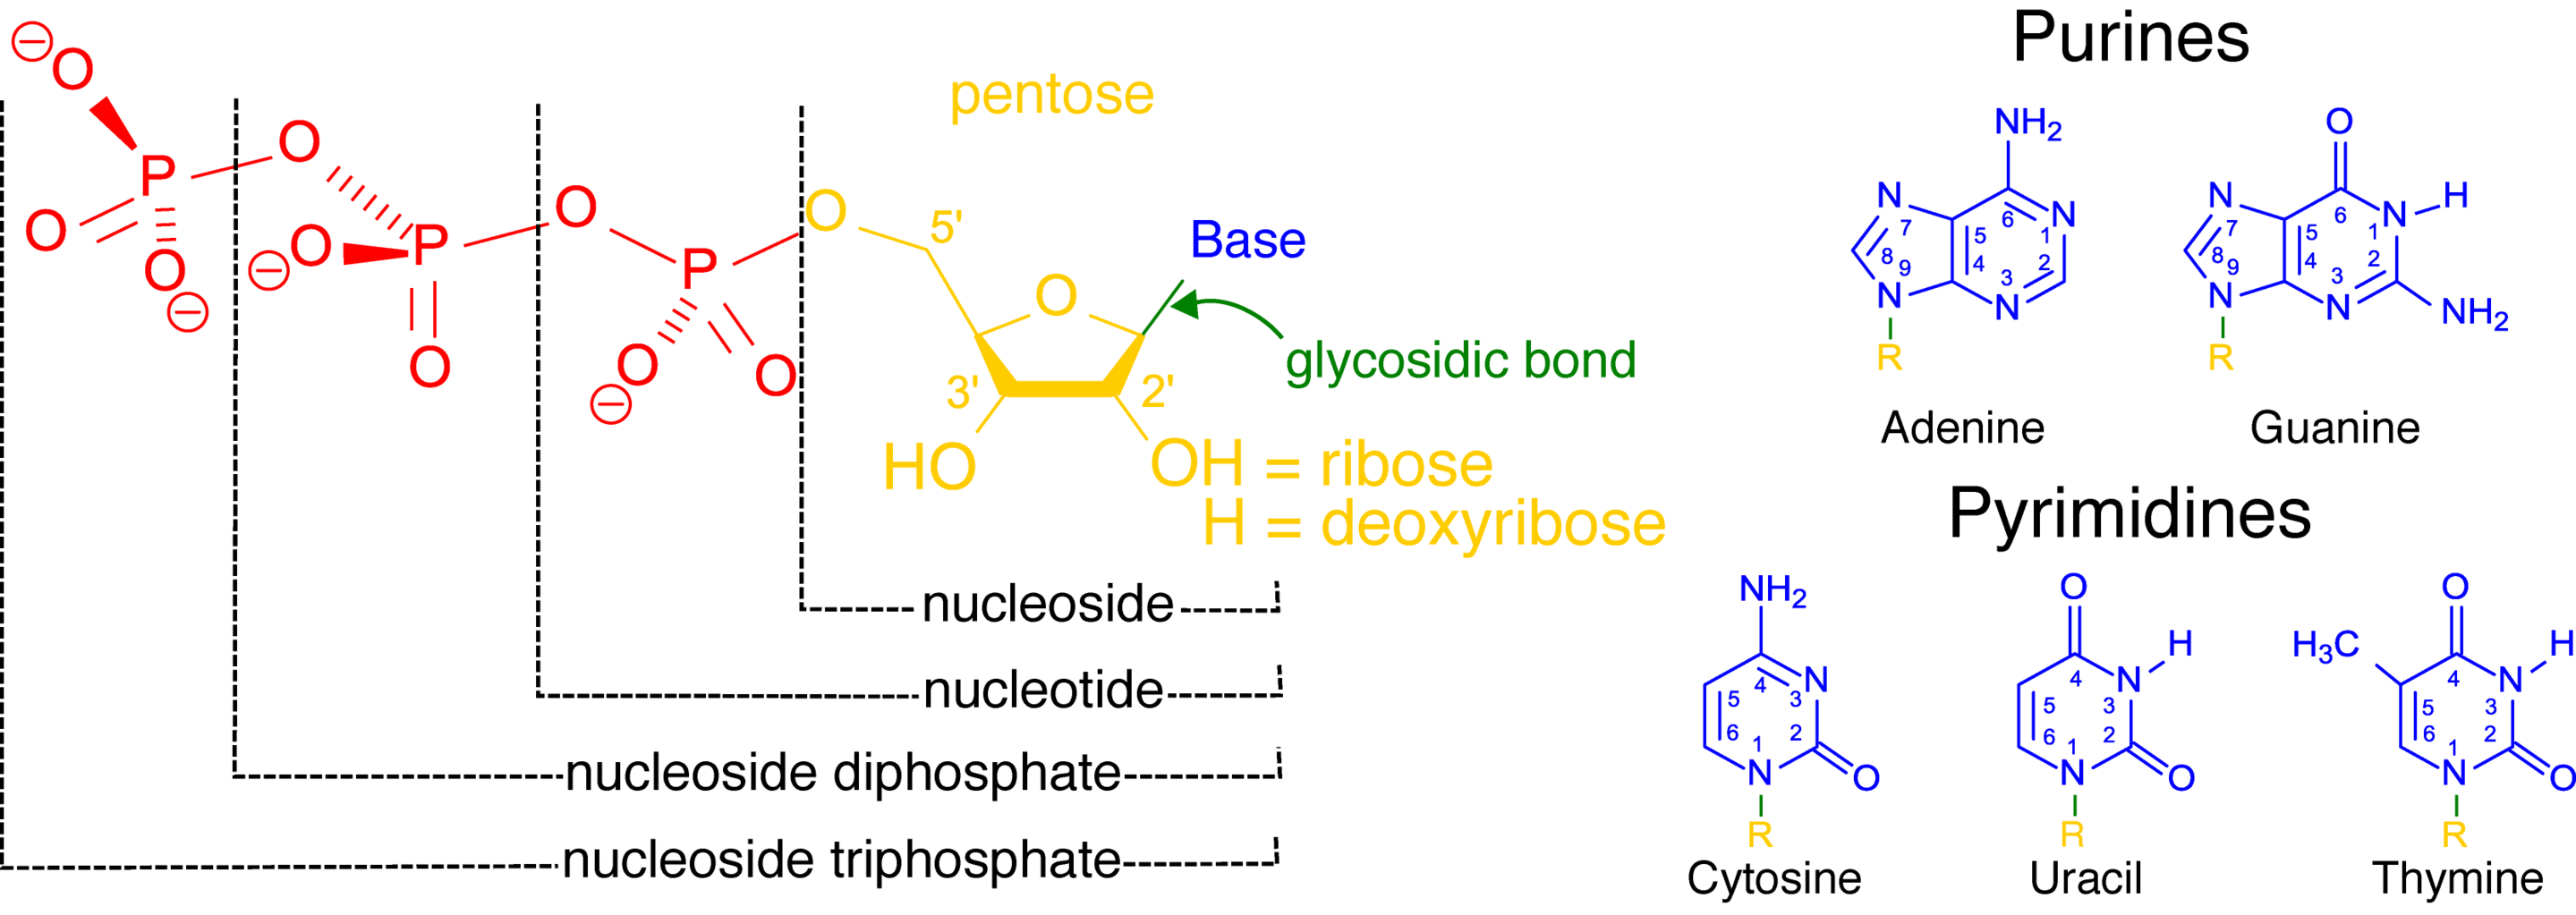
\includegraphics[width=1\textwidth]{images/Nucleotides.png}\\[.2in]
\caption{RNA and DNA} 
\end{figure}

\begin{itemize}[noitemsep]
    \item \bd{A} Adenine
    \item \bd{G} Guanine
    \item \bd{C} Cytosine
    \item \bd{U} Uracil
    \item \bd{T} Thymine
\end{itemize}
Nucleoside = Sugar + Base (the information carrier)
\begin{itemize}
    \item DNA: sugar is deoxyribose\footnote{a sugar derived from ribose by replacement of a hydroxyl group by hydrogen.}; bases are A,C,G,T - relatively stable.
    \item RNA: sugar is ribose\footnote{a sugar of the pentose class which occurs widely in nature as a constituent of nucleosides and several vitamins and enzymes.}; bases are A,C,G,U - relatively unstable.
\end{itemize}
The nucleotide triphosphate forms are the building block.

\section{RNA structural diversity}
\udl{A single-stranded RNA molecule can base-pair with itself}
to form structures that are biochemically important. It is quite possible that RNA molecules or something similar are the origin of life.\\[.2in]
Examples: Hammerhead ribozyme\footnote{an RNA-cutting RNA enzyme} and transfer RNA.

\section{Amino acid structure}
\begin{figure}[h]
    \centering
    \chemfig{N(-[3]H)(-[5]H)-C(-[2]R)(-[6]H)-C(=[1]O)(-[-1]OH)}
    \caption{Amino acid structure}
\end{figure}
\begin{itemize}[noitemsep]
    \item R-group (side chain)  
    \item Amino group: N terminus
    \item Alpha carbon
    \item Carboxyl group: C terminus
\end{itemize}
Amino acids: modular protein sub-units: 20 amino acid structures.
\begin{enumerate}[itemsep=0mm]
    \item Amino acids with hydrophobic side chains
    \item Amino acids with hydophilic side chains
    \item Amino acids with intermediate side chains
\end{enumerate}

\section{The peptide bond}
The N terminus (Amino terminus) is the start of a protein and the C terminus (Carboxy terminus) the end.
\begin{scheme}[h]
    \centering
    \schemestart
        $2$ \chemname{
            \chemfig{N(-[3]H)(-[5]H)-C(-[2]R)(-[6]H)-C(=[1]O)(-[-1]OH)}
        }{Amino acid}
        \arrow(.mid east--.mid west){<=>[Dehydration]}
        \chemname{
            \chemfig{N(-[3]H)(-[5]H)-C(-[2]H)(-[6]R)-C(=[2]O)-N(-[-2]H)-C(-[2]H)(-[6]R)-C(=[1]O)(-[-1]OH)}
        }{Pipetide group}
        \+
        \[ \text{H}_2\text{O} \]
    \schemestop
    \caption{The condensation reaction to generate a pipetide group}
    \label{scm:tsester}
\end{scheme}


\section{Protein structural hierarchy}

\bd{Primary structure}: sequence of amino-acids: determines the final form and function (peptide bonds)\\[.1in]
\bd{Primary structure}: sequence of alpha-helices, beta-sheets (hydrogen bonding)\\[.1in]
\bd{Tertiary structure}: overall 3D fold (disulphide bonds, ionic bonds, hydrogen bonds...)\\[.1in]
\bd{Quaternary structure}: complex of proteins

\section{Information flow: the Central Dogma of molecular biology}
Francis Crick (1958) raised the idea that the information flows from the DNA to RNA, and then to the Proteins.
\begin{figure}[h]
\centering
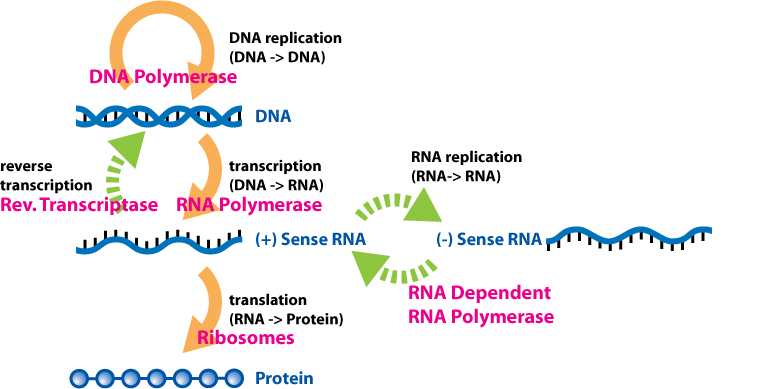
\includegraphics[width=0.8\textwidth]{images/Extended_Central_Dogma_with_Enzymes.jpg}\\[.2in]
\caption{Demonstration of Central Dogma} 
\end{figure}
\begin{enumerate}
    \item DNA replication via DNA Polymerase\footnote{catalyse the synthesis of DNA molecules from nucleoside triphosphates, the molecular precursors of DNA} (DNA $\rightarrow$ DNA)
    \item Transcription via RNA polymeras\footnote{an enzyme that synthesises RNA from a DNA template} (DNA $\rightarrow$ RNA)
    \item Translation via Ribosomes\footnote{Ribosomes link amino acids together in the order specified by the codons of messenger RNA (mRNA) molecules to form polypeptide chains.} (DNA $\rightarrow$ Protein)
\end{enumerate}

\subsection{DNA polymerase}
\begin{itemize}
    \item DNA replication is catalysed by DNA polymerase.
    \item Polymerisation is in the 5' $\rightarrow$ 3' direction.
    \item DNA polymerase starts from an existing 3'-hydroxyl group, i.e. it needs a "\textit{primer}".
    \item The primer can be a \udl{synthetic DNA molecule} that anneals to a template through \textit{complementary base pairing}.
\end{itemize}

\subsection{Transcriptions and Translations}
\bd{Transcription} \\ [.1in]
Transcription is re-writing in a similar alphabet.
\begin{itemize}
    \item Catalysed by RNA polymerase enzyme from 5' to 3' direction.
    \item Template strand is the bottom strand (\textit{coding strand}).
    \item RNA uses Uracil (U) instead of T.
    \item RNA has a 2'hydroxyl group (so ribose not deoxyribose)
    \item The RNA molecule is called a transcript. The transcript of a protein-coding RNA is called a messenger RNA (mRNA).
\end{itemize}
Convention: for a gene drawn, we write the sequence of the \udl{top strand}. We need to reverse-complement genes on the bottom strand.\\[.2in]
\bd{Translation} \\ [.1in]
Translation is recoding: one \textit{codon} = 3 bases. Therefore, 64 codons map to 20 amino acids + 3 stop codons. \udl{Translation is carried out by the ribosome.} The ribosome is a giant RNA/protein complex that has two subunits.
\begin{itemize}
    \item The mRNA is read 5' $\rightarrow$ 3'.
    \item The protein is sythesised N terminus $\rightarrow$ C terminus.
    \item The redundancy of 3 bases is removed by a multiple-to-one mapping from codons to amino acids.
    \item The tRNA carries the Amino acid and with \udl{anticodon loop} on the other side which matches the mRNA. 
\end{itemize}
Enzymes called \udl{amino-acly rRNA synthetases} 'charge' tRNAs by attaching the correct amino-acid for the anticodon.
\begin{itemize}
    \item Certain tRNAs recognise more than one codon by means of the last base "wobbling" (forming atypical base pairs).
    \item tRNA synthetases have been evolved that can mis-charge tRNAs with exotic amino-acids.
\end{itemize}
Epigenetics and prions make the picture more complicated but the central dogma is still central to life.
 
\chapter{Gene Cloning}

\section{Genetic Engineering Applications}
\bd{Plants}\\[.1in]
A wide variety of different alterations has been made plants affecting not just their yields but also multiple resistances.\\[.2in]
\bd{Pharmaceutical industry}\\[.1in]
Product like recombinant insulin or variants, recombinant GCSF\footnote{prevents infections during cancer
chemotherapy}, humanising therapeutic antibodies are developed.\\[.2in]
\bd{Research}
\begin{enumerate}[noitemsep]
    \item \udl{molecular biology} enzyme production, time/location functional studies
    \item developmental biology: GFP (and related) fusion proteins
    \item gene knock-out/in libraries
\end{enumerate}

\section{Cloning Vectors for use in E. coli}
Derived from plasmids\footnote{a genetic structure in a cell that can replicate independently of the chromosomes} and bacteriophage\footnote{phage for short: a virus which parasitizes a bacterium by infecting it and reproducing inside it.}. Important parts includes:
\begin{itemize}[noitemsep]
    \item origin of replication
    \item selectable marker
    \item multiple cloning site (MCS)
\end{itemize}

\subsection{Typical workflow for making recombinant DNA}
\begin{figure}[h]
\centering
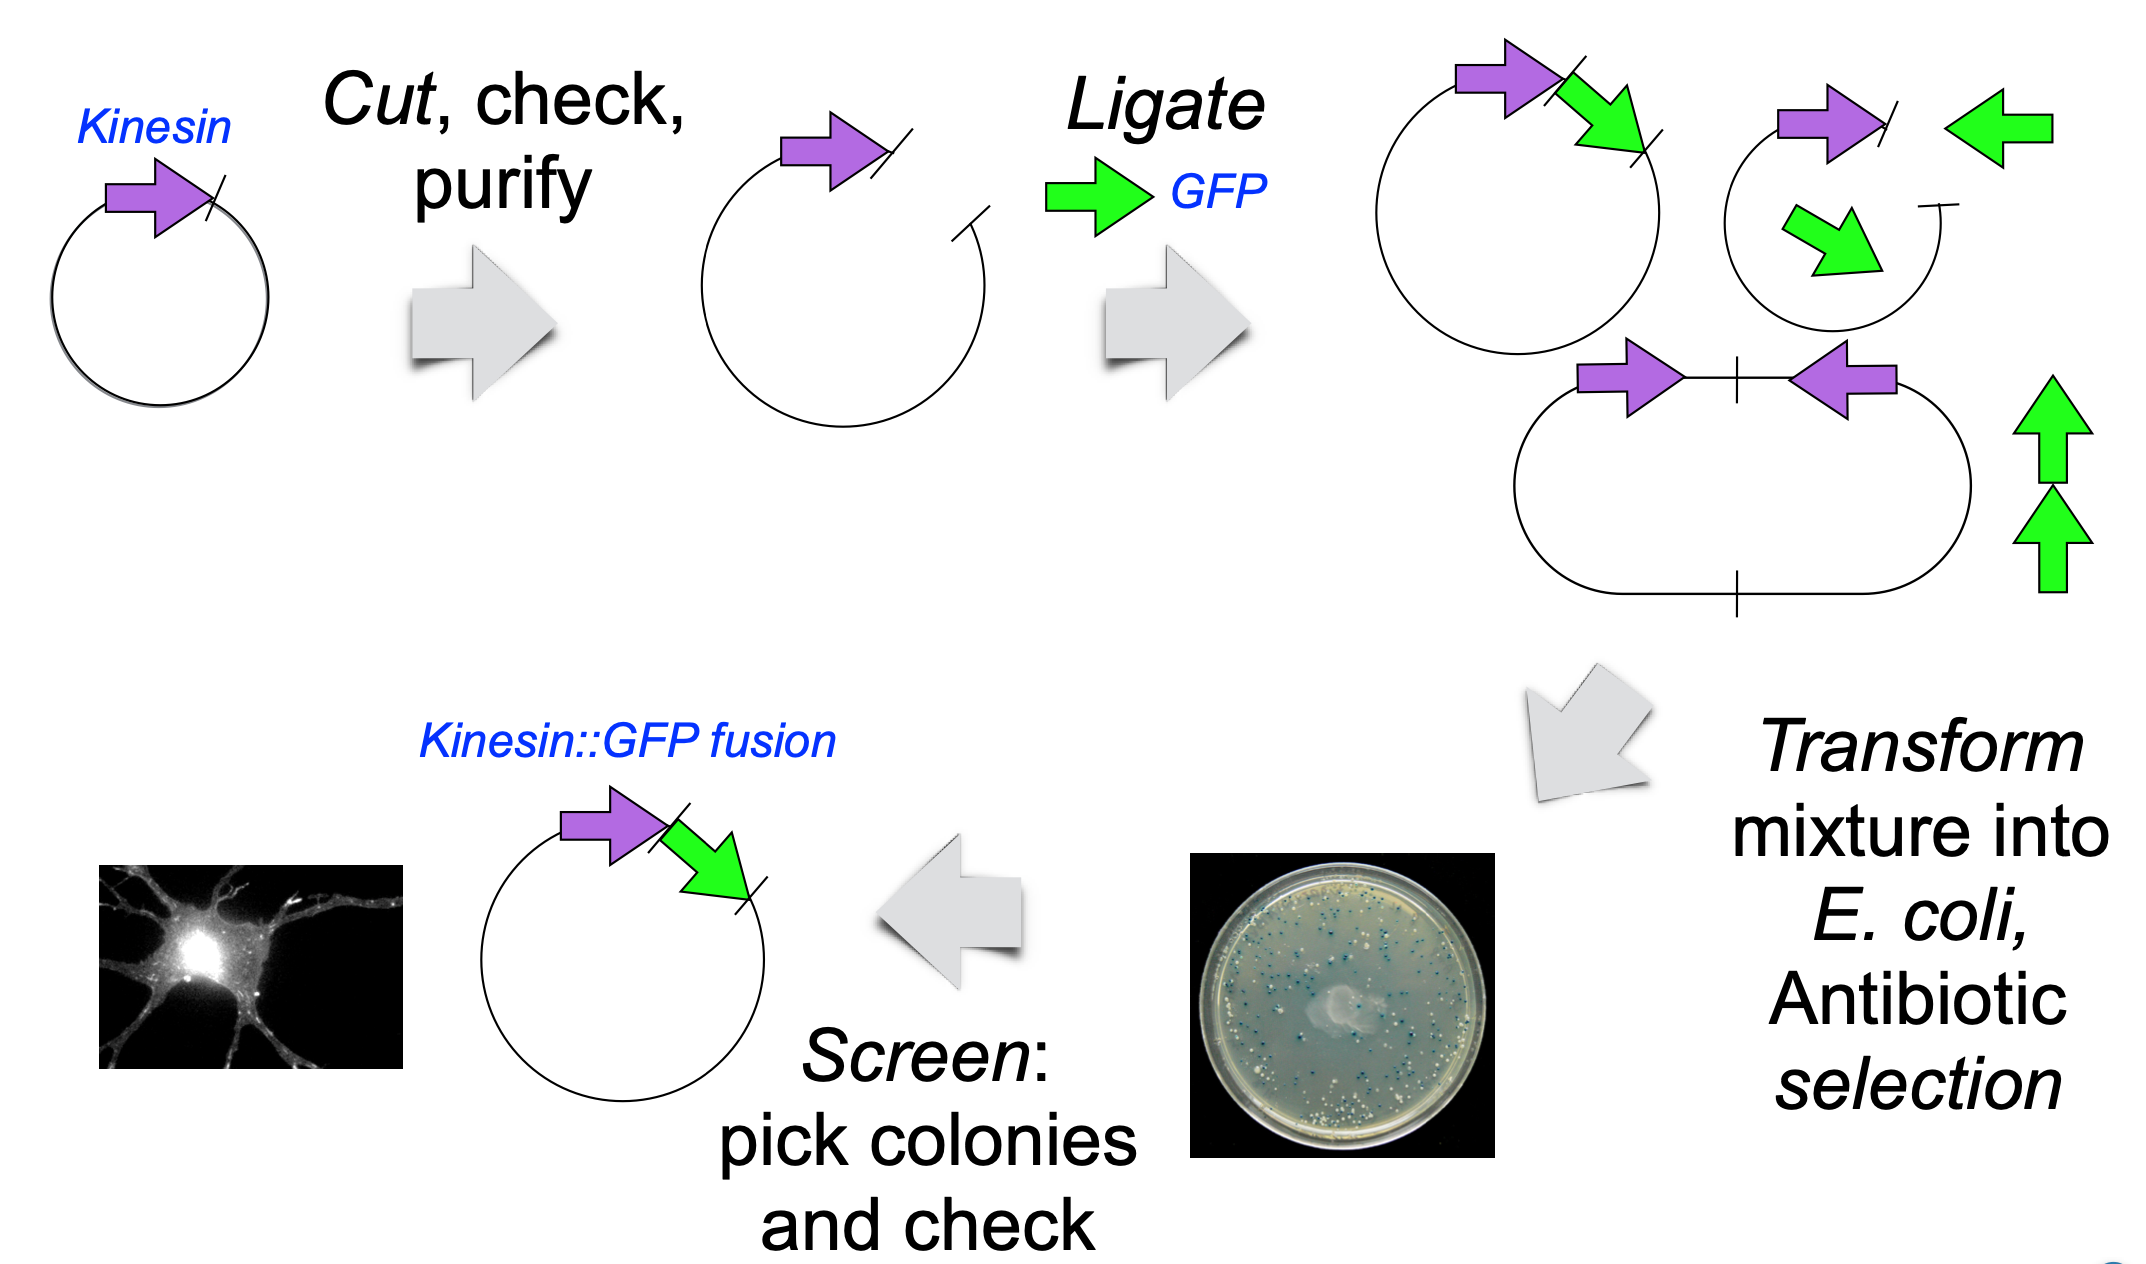
\includegraphics[width=0.8\textwidth]{images/lecture4-1.png}\\[.2in]
\caption{Typical workflow for making recombinant DNA} 
\end{figure}
\subsection{Distinguish between single clones and libraries of clones}
\bd{Make one clone}\\
For example, fusing one gene (GFP) to another (kinesin)\\[.2in]
\bd{Making a library of clones}\\
For example, cloning a set of fragments representing all genes expressed in a tissue.
\subsection{Bacterial plasmids and phage}
Recall prokaryotic horizontal gene transfer via conjugation (moves plasmids) or transduction by phage.
\subsection{Selectable markers}
\begin{itemize}[noitemsep]
    \item Ampicillin: amp\textsuperscript{r}
    \item Kanamycin: kan\textsuperscript{r}
    \item Tetracyclines: tet\textsuperscript{r}
    \item Chloramphenicol: cap\textsuperscript{r}
\end{itemize}
\subsection{Cutting DNA: Restriction enzymes}
\bd{Restriction enzymes cut DNA}
\begin{itemize}
    \item It cuts \udl{specific sequence motif}\footnote{distinctive sequence on a protein or DNA, having a three-dimensional structure that allows binding interactions to occur.}.
    \item the motif is often \udl{palindromic}.
    \item Bacterial defence mechanism: restriction enzymes only cut unmethylated DNA, for example, invading viral DNA.
    \item Chromosomal DNA is protected by a DNA methylase that methylates the motif.
\end{itemize}
\bd{Sticky and Blunt cut}
\begin{enumerate}
    \item \bd{Blunt Cut}: The cuts of the DNA strand are opposite to each other.
    \item \bd{Sticky Overhang}: After cutting and separation, there is a short 4 base extension.
    \begin{enumerate}
        \item Sticky: 5' overhang (extension on 3')
        \item Sticky: 3' overhang (extension on 5')
    \end{enumerate}
\end{enumerate}
\subsection{Pasting DNA: DNA Ligase}
\begin{itemize} 
    \item DNA ligase rejoins cut DNA strands.
    \item Ligase works on \udl{correctly base-paired} sticky ends.
    \item Ligase can also join blunt-ended DNA, but less efficiently.
\end{itemize}
\subsection{Recombinant DNA}
The figure \ref{Fig4-2} illustrates the sequence dependent cleavage and assembly of DNA.
\begin{figure}[h]
\centering
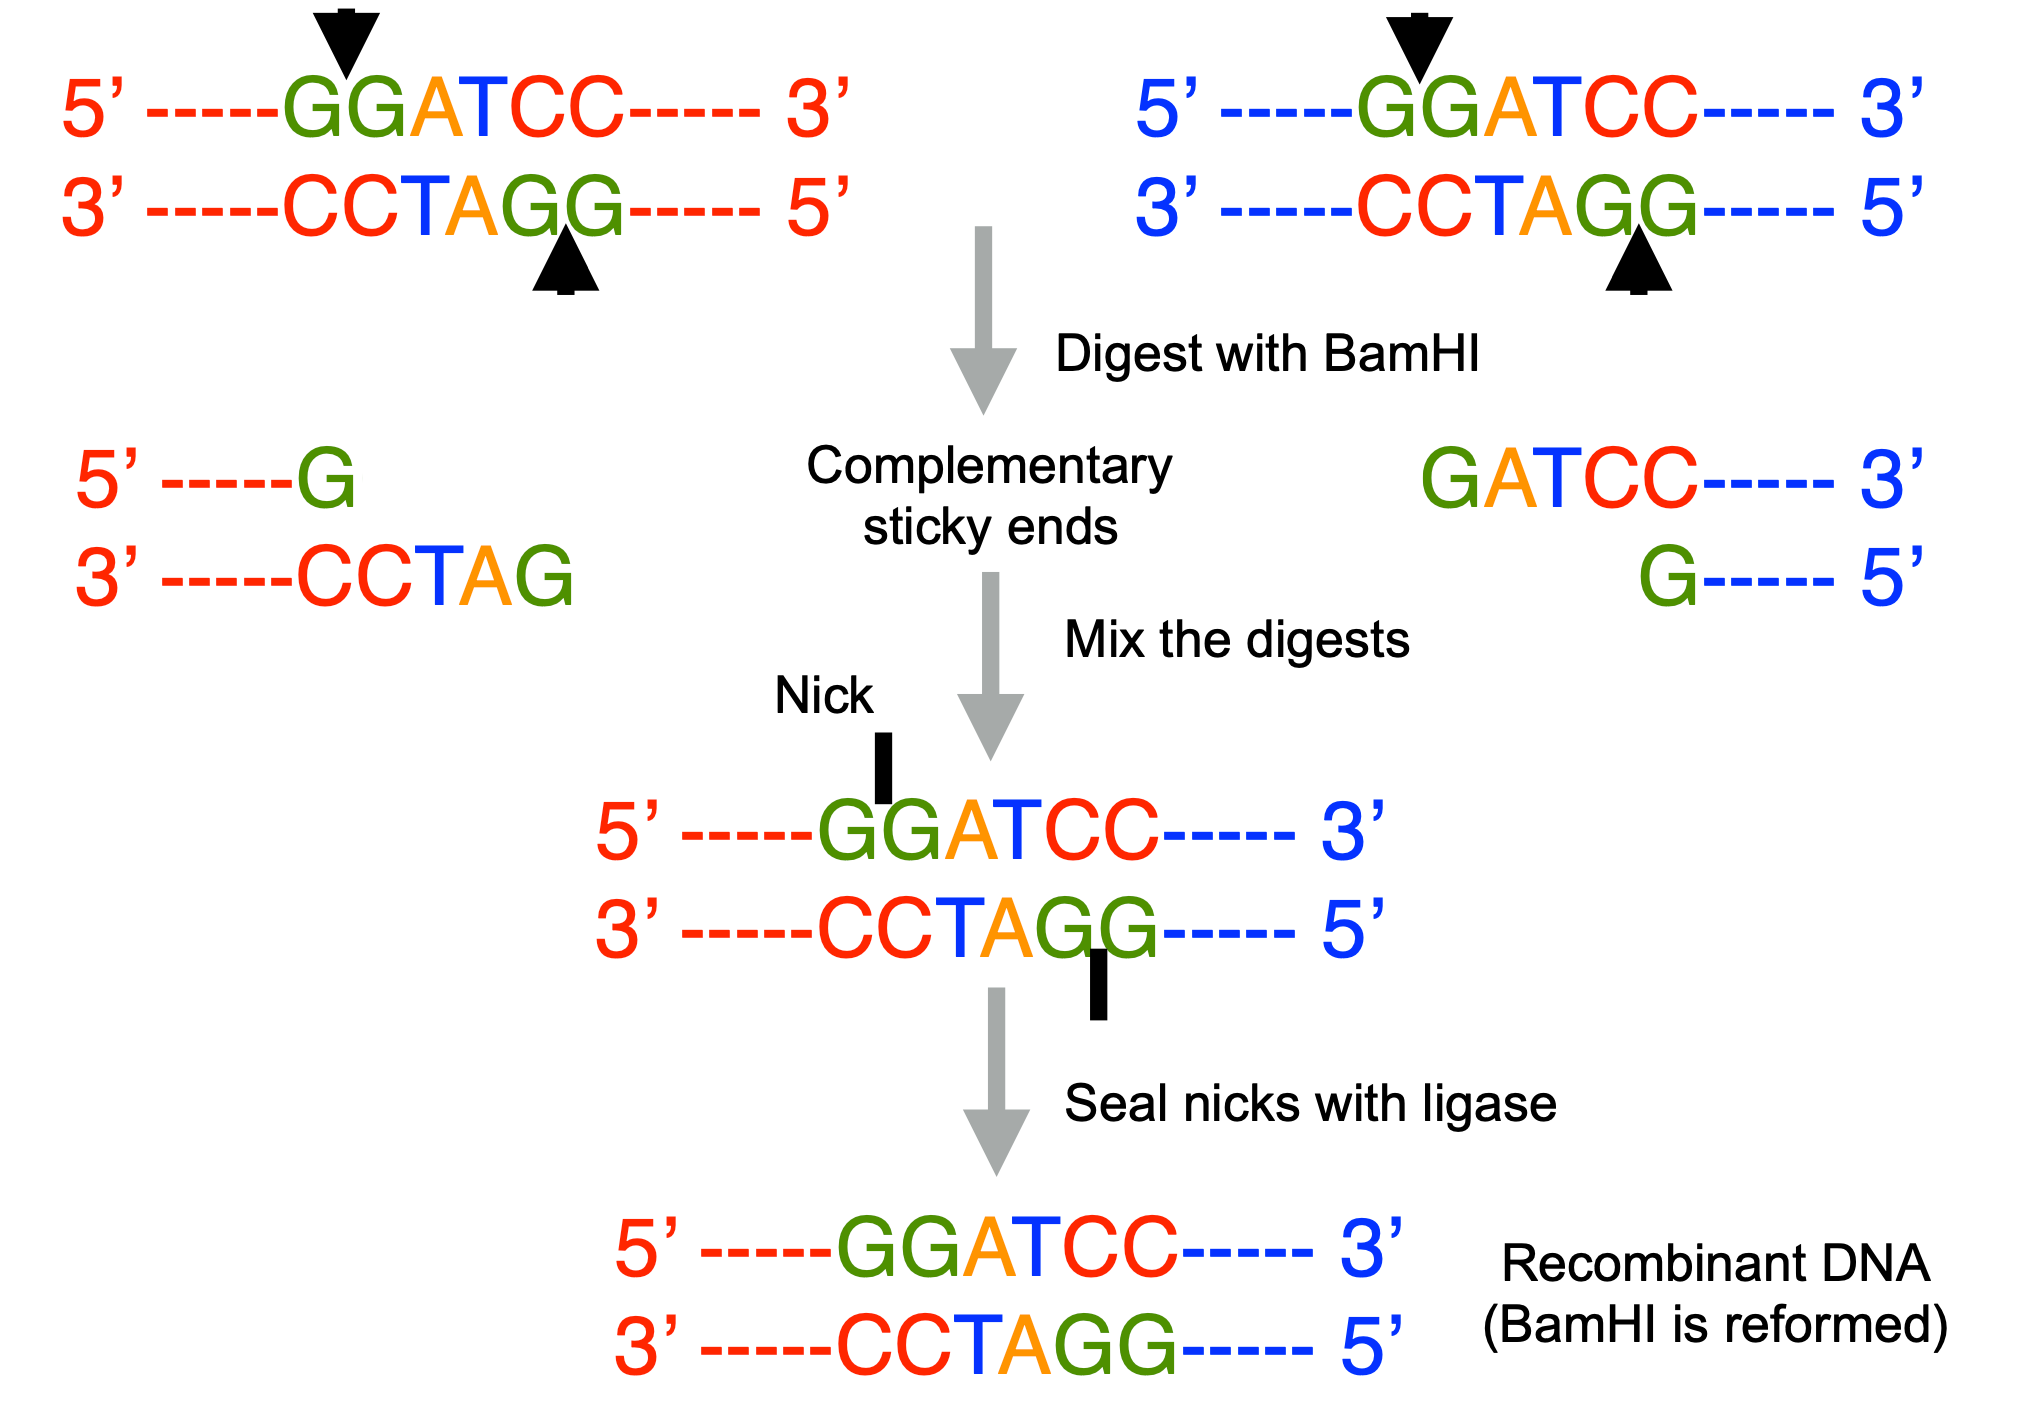
\includegraphics[width=0.8\textwidth]{images/lecture4-2.png}\\[.2in]
\caption{Sequence dependent cleavage and assembly of DNA} 
\label{Fig4-2}
\end{figure}
\subsection{Purifying DNA: Gel elecytophoresis}
\begin{itemize}
    \item DNA is negatively charged in solution at pH=7 to 8.
    \item DNA will \udl{migrate in an electric field}.
    \item Smaller molecules migrate more rapidly in agarose or polyacrylamide gels.
    \item DNA can be visualised in UV light by staining with dyes like \udl{ethidium bromide}.
    \item Can cut out bands from gel in order to purify DNA fragments.
\end{itemize}
\subsection{Inserting DNA into cells: bacterial transformation}
There are two ways to insert DNA liagtion mixture into cells:
\begin{enumerate} 
    \item Chemical transformation:
    \begin{itemize}
        \item wash cells in chilled CaCl\textsubscript{2} to permeabilise the membrane
        \item $ 42\degree$C heat shock to promote DNA uptake
    \end{itemize}
    \item Transformation by electroporation
    \begin{itemize}
        \item wash calls in water (to remove ions)
        \item 5-20kV/cm shock promotes DNA uptake
    \end{itemize}
\end{enumerate}
Both methods are followed by a \udl{recovery period} in rich medium to allow time for \udl{expression of the antibiotic resistance gene}. The cells are plated on \udl{agar plates} containing \udl{nutrients} plus \udl{antibiotics}.
\subsection{Bacterial Cell Culture}
Growth on nutrient agar plates allows \udl{isolation of \textit{colonies}}: a colony is a clone of cells that has grown from one cell.\\[.1in]
Individual colonies are picked into \udl{liquid medium} for growth before preparing DNA. Large scale cultures (thousands to millions of litres) are used for industrial production. Good sterile technique is required.

\subsection{Summary: cloning steps}
Cloning vecors allow foreign DNA to be cloned/amplifies
\begin{enumerate}[itemsep=0mm]
    \item \bd{cut} vector, foreign DNA with compatible restriction enzymes
    \item \bd{isolate} fragments of interest via gel electriphoresis
    \item \bd{ligate} foreign DNA into vector
    \item \bd{transform} recombinant DNA into host (typically \textit{E. coli})
    \item \bd{select} for growth of transformed bacteria
    \item \bd{screen} colonies for correct DNA arrangement
\end{enumerate}
Limitations are
\begin{enumerate} [itemsep=0mm]
    \item Expensive: it requires very highly purifies enzymes.
    \item Chance/Need more control: it requires restriction sites in the right place.
\end{enumerate}

\section{CRISPR/cas9}
\subsection{CRISPR/cas9: programmable recognition}
The gRNA specificity is 20 bases, which ensures the accuracy of editing. Target must be followed by
protospacer adjacent motif (PAM) = NGG for S. pyogenes Cas9.\\[.2in]
\begin{figure}[h]
\centering
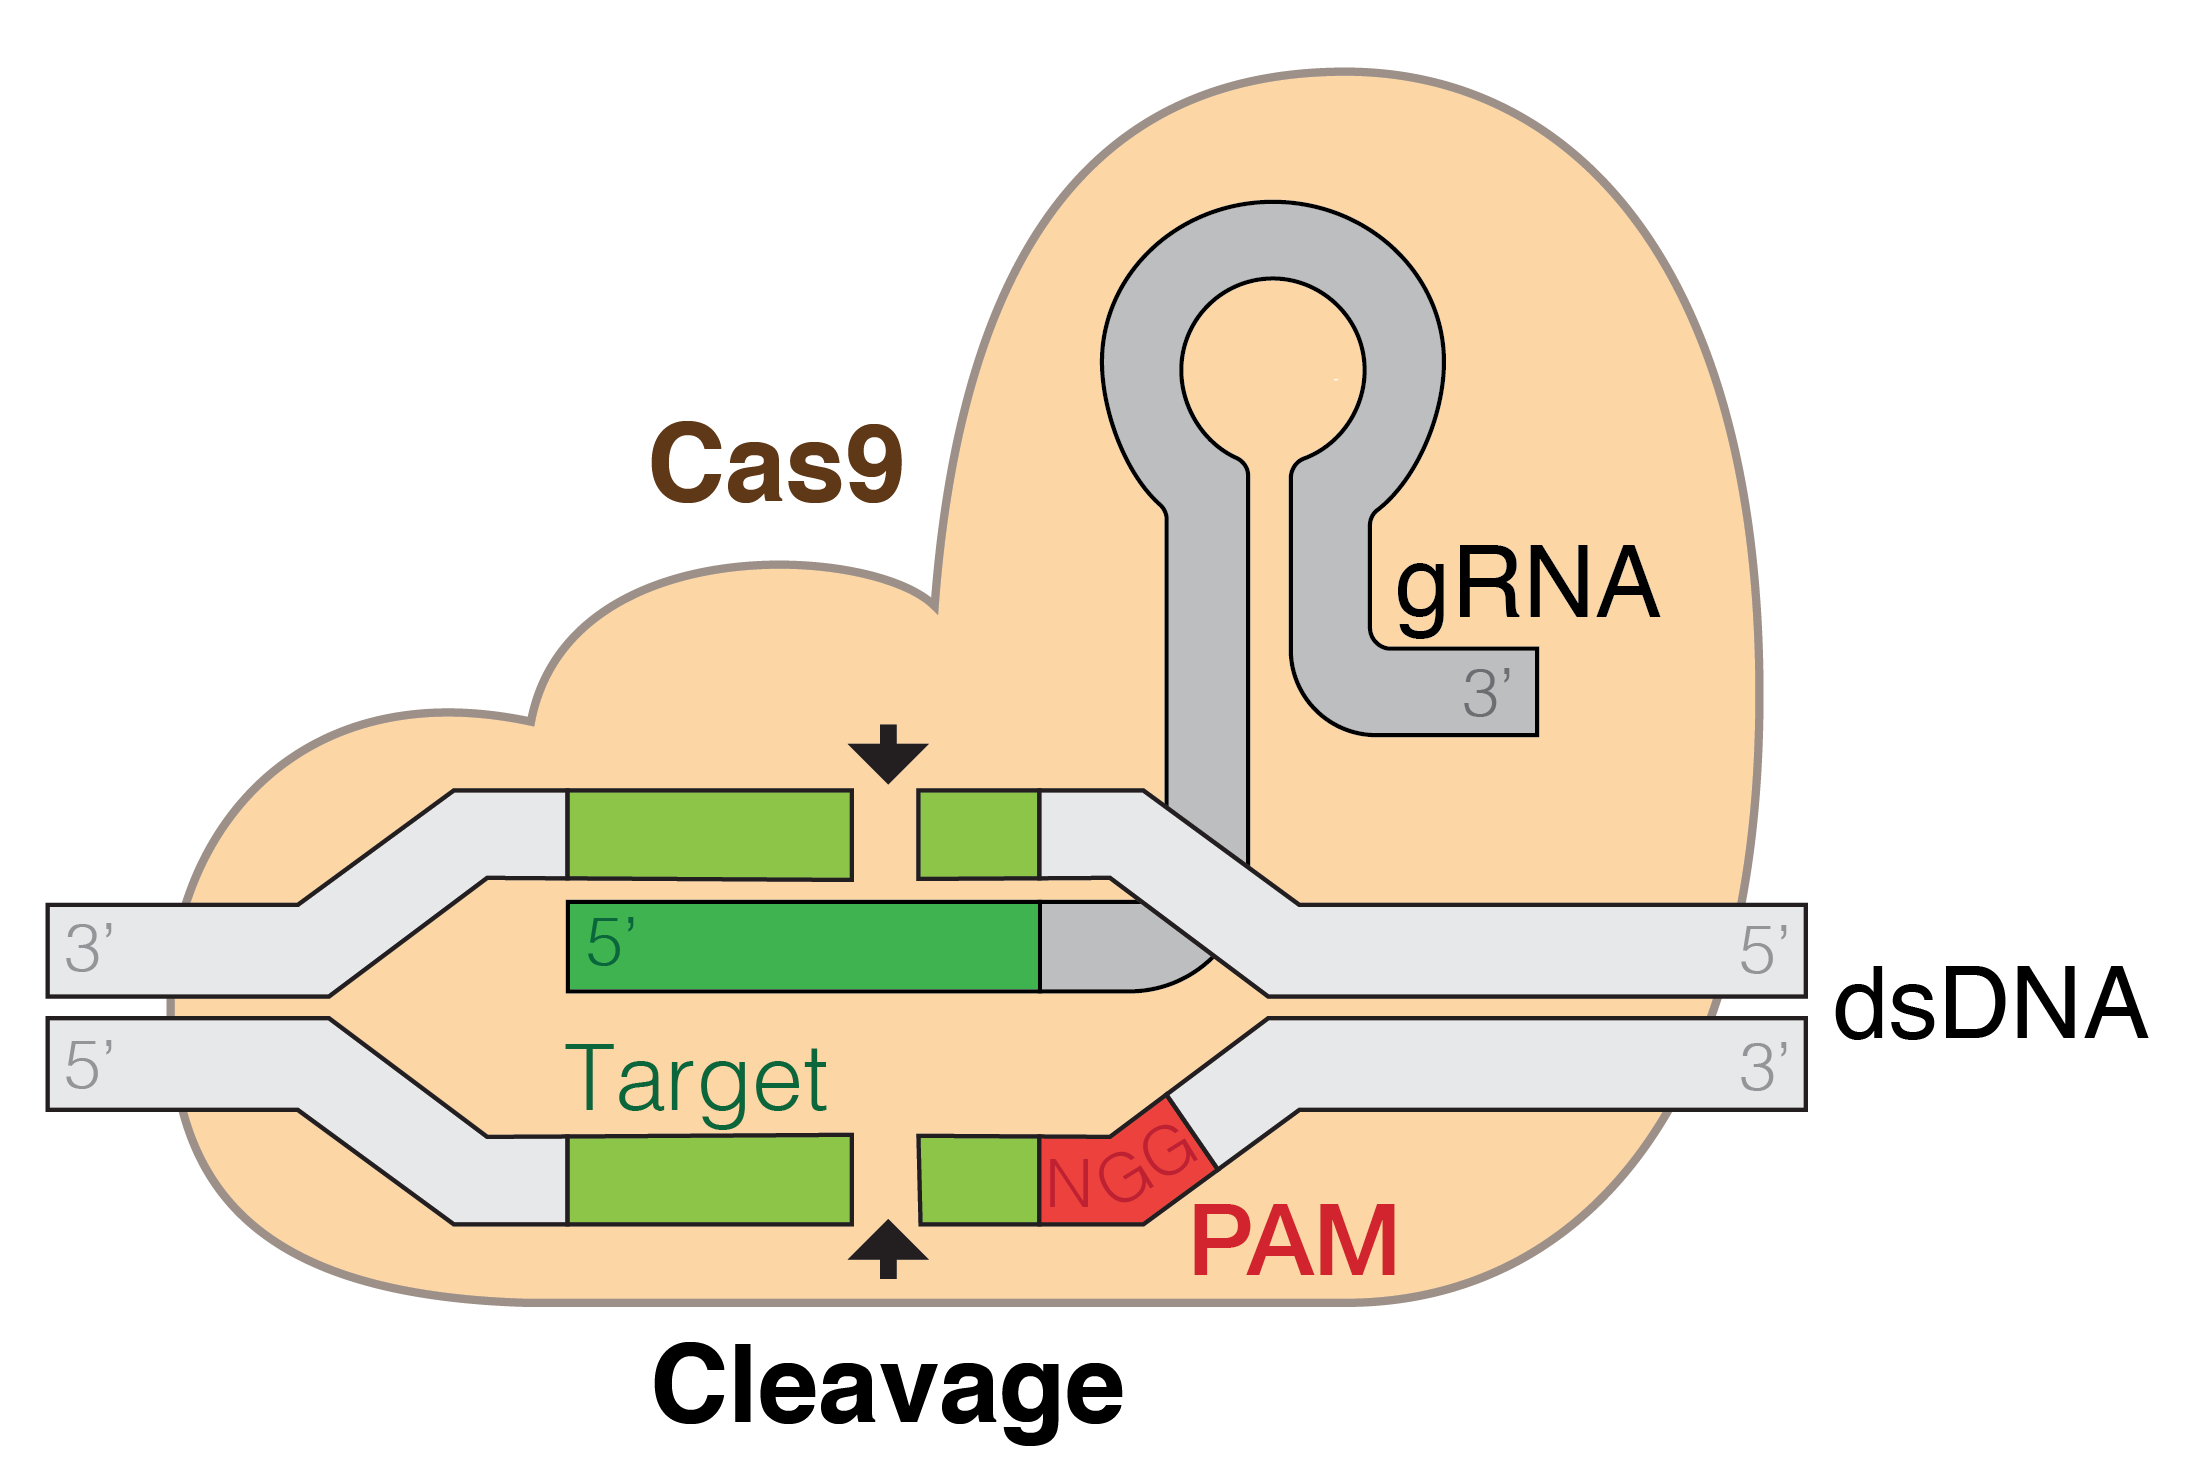
\includegraphics[width=0.6\textwidth]{images/GRNA-Cas9.png}\\[.2in]
\caption{CRISPR/cas9}
\end{figure}
In the Non-Homologous End Joining (NHEJ) (figure \ref{repair}), one can knock out the gene by making a cut at the specific location and causes deletion and insertions which disable the gene.\\[.2in]
Even more powerfully, by transforming a piece of \udl{linear DNA} containing the desired changes. If the linear DNA has sequence similarities on either side of the cut side, the repair machinery will do the Homology Directed Repair (HDR) by reference with the linear DNA inserted. This is why it is very efficient in editing the genes.
\begin{figure}[h]
\centering
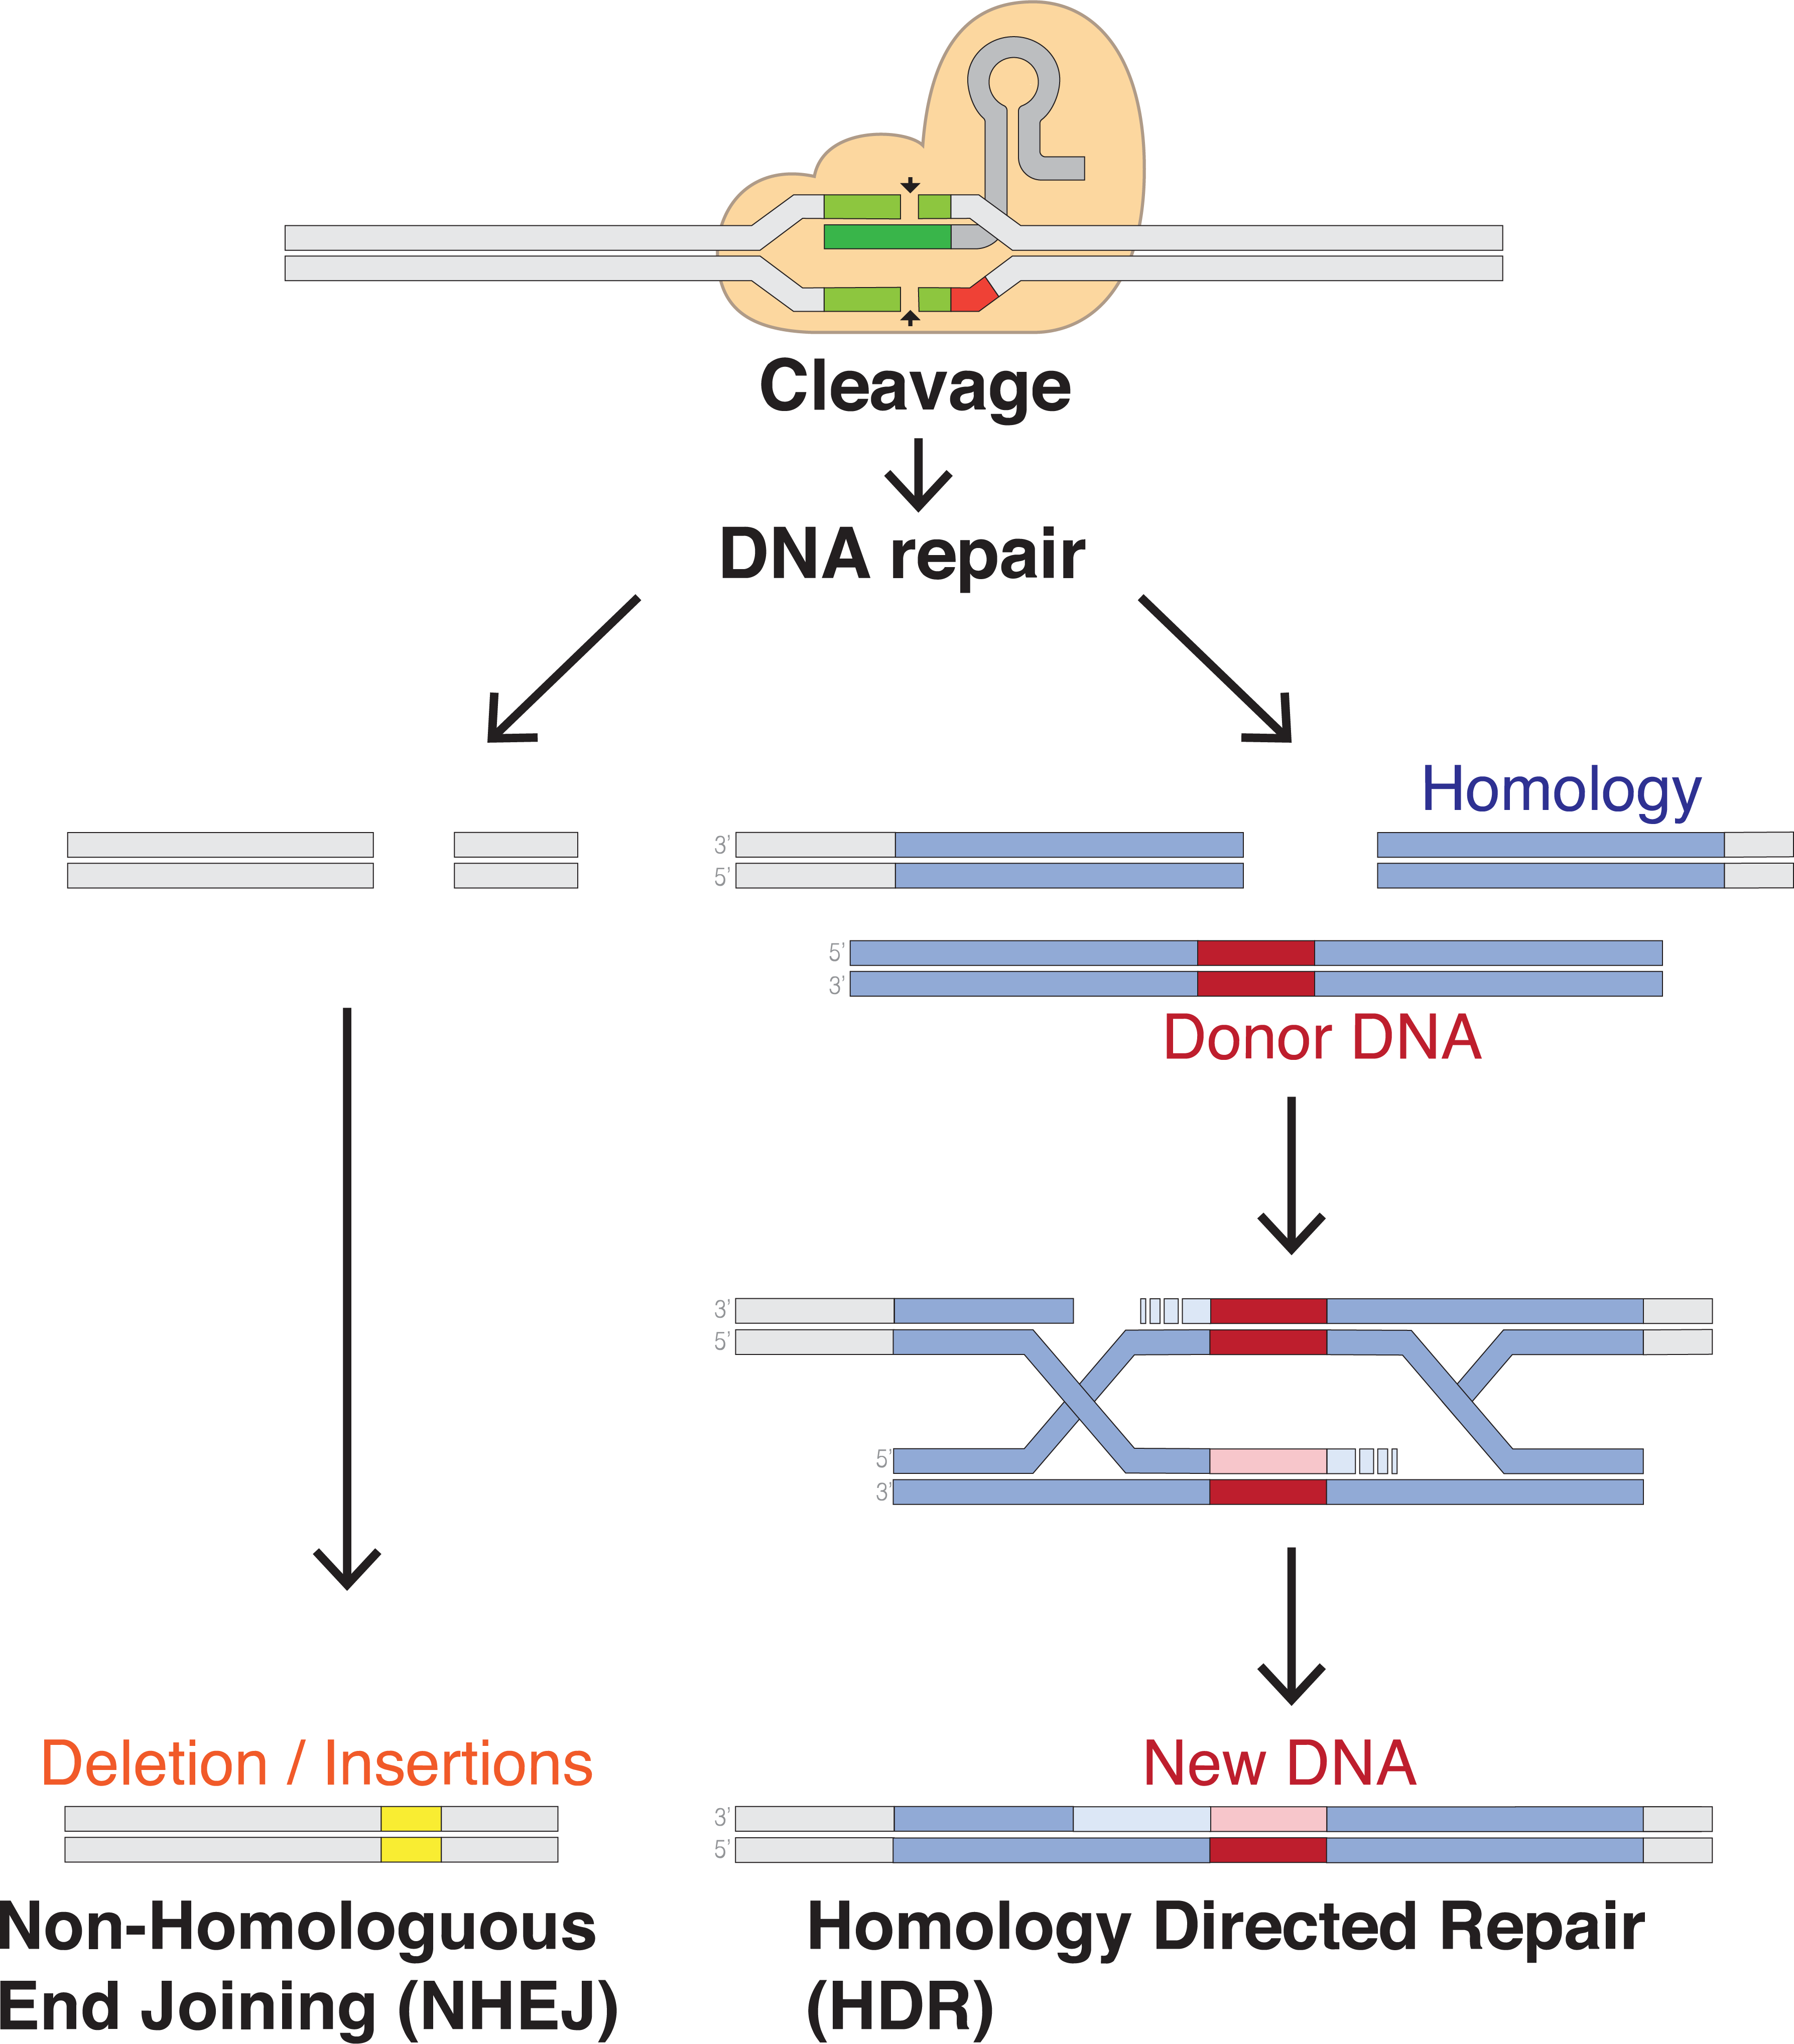
\includegraphics[width=0.4\textwidth]{images/DNA_Repair.png}\\[.2in]
\caption{DNA repair with CRISPR/cas9}
\label{repair}\\[.2in]
\end{figure}
\subsection{Application areas}
\begin{itemize}
    \item programmable sequence-specific nucleases
    \item simpler genome editing: potential to reverse genetic diseases
    \item programmable transcription regulators
    \item systematic whole-genome mutagensis (allows functional screens)
    \item transgenic mice much more quickly
    \item dCas9 mutant does not cut (figure \ref{dCas9})
\end{itemize}
\begin{figure}[h]
\centering
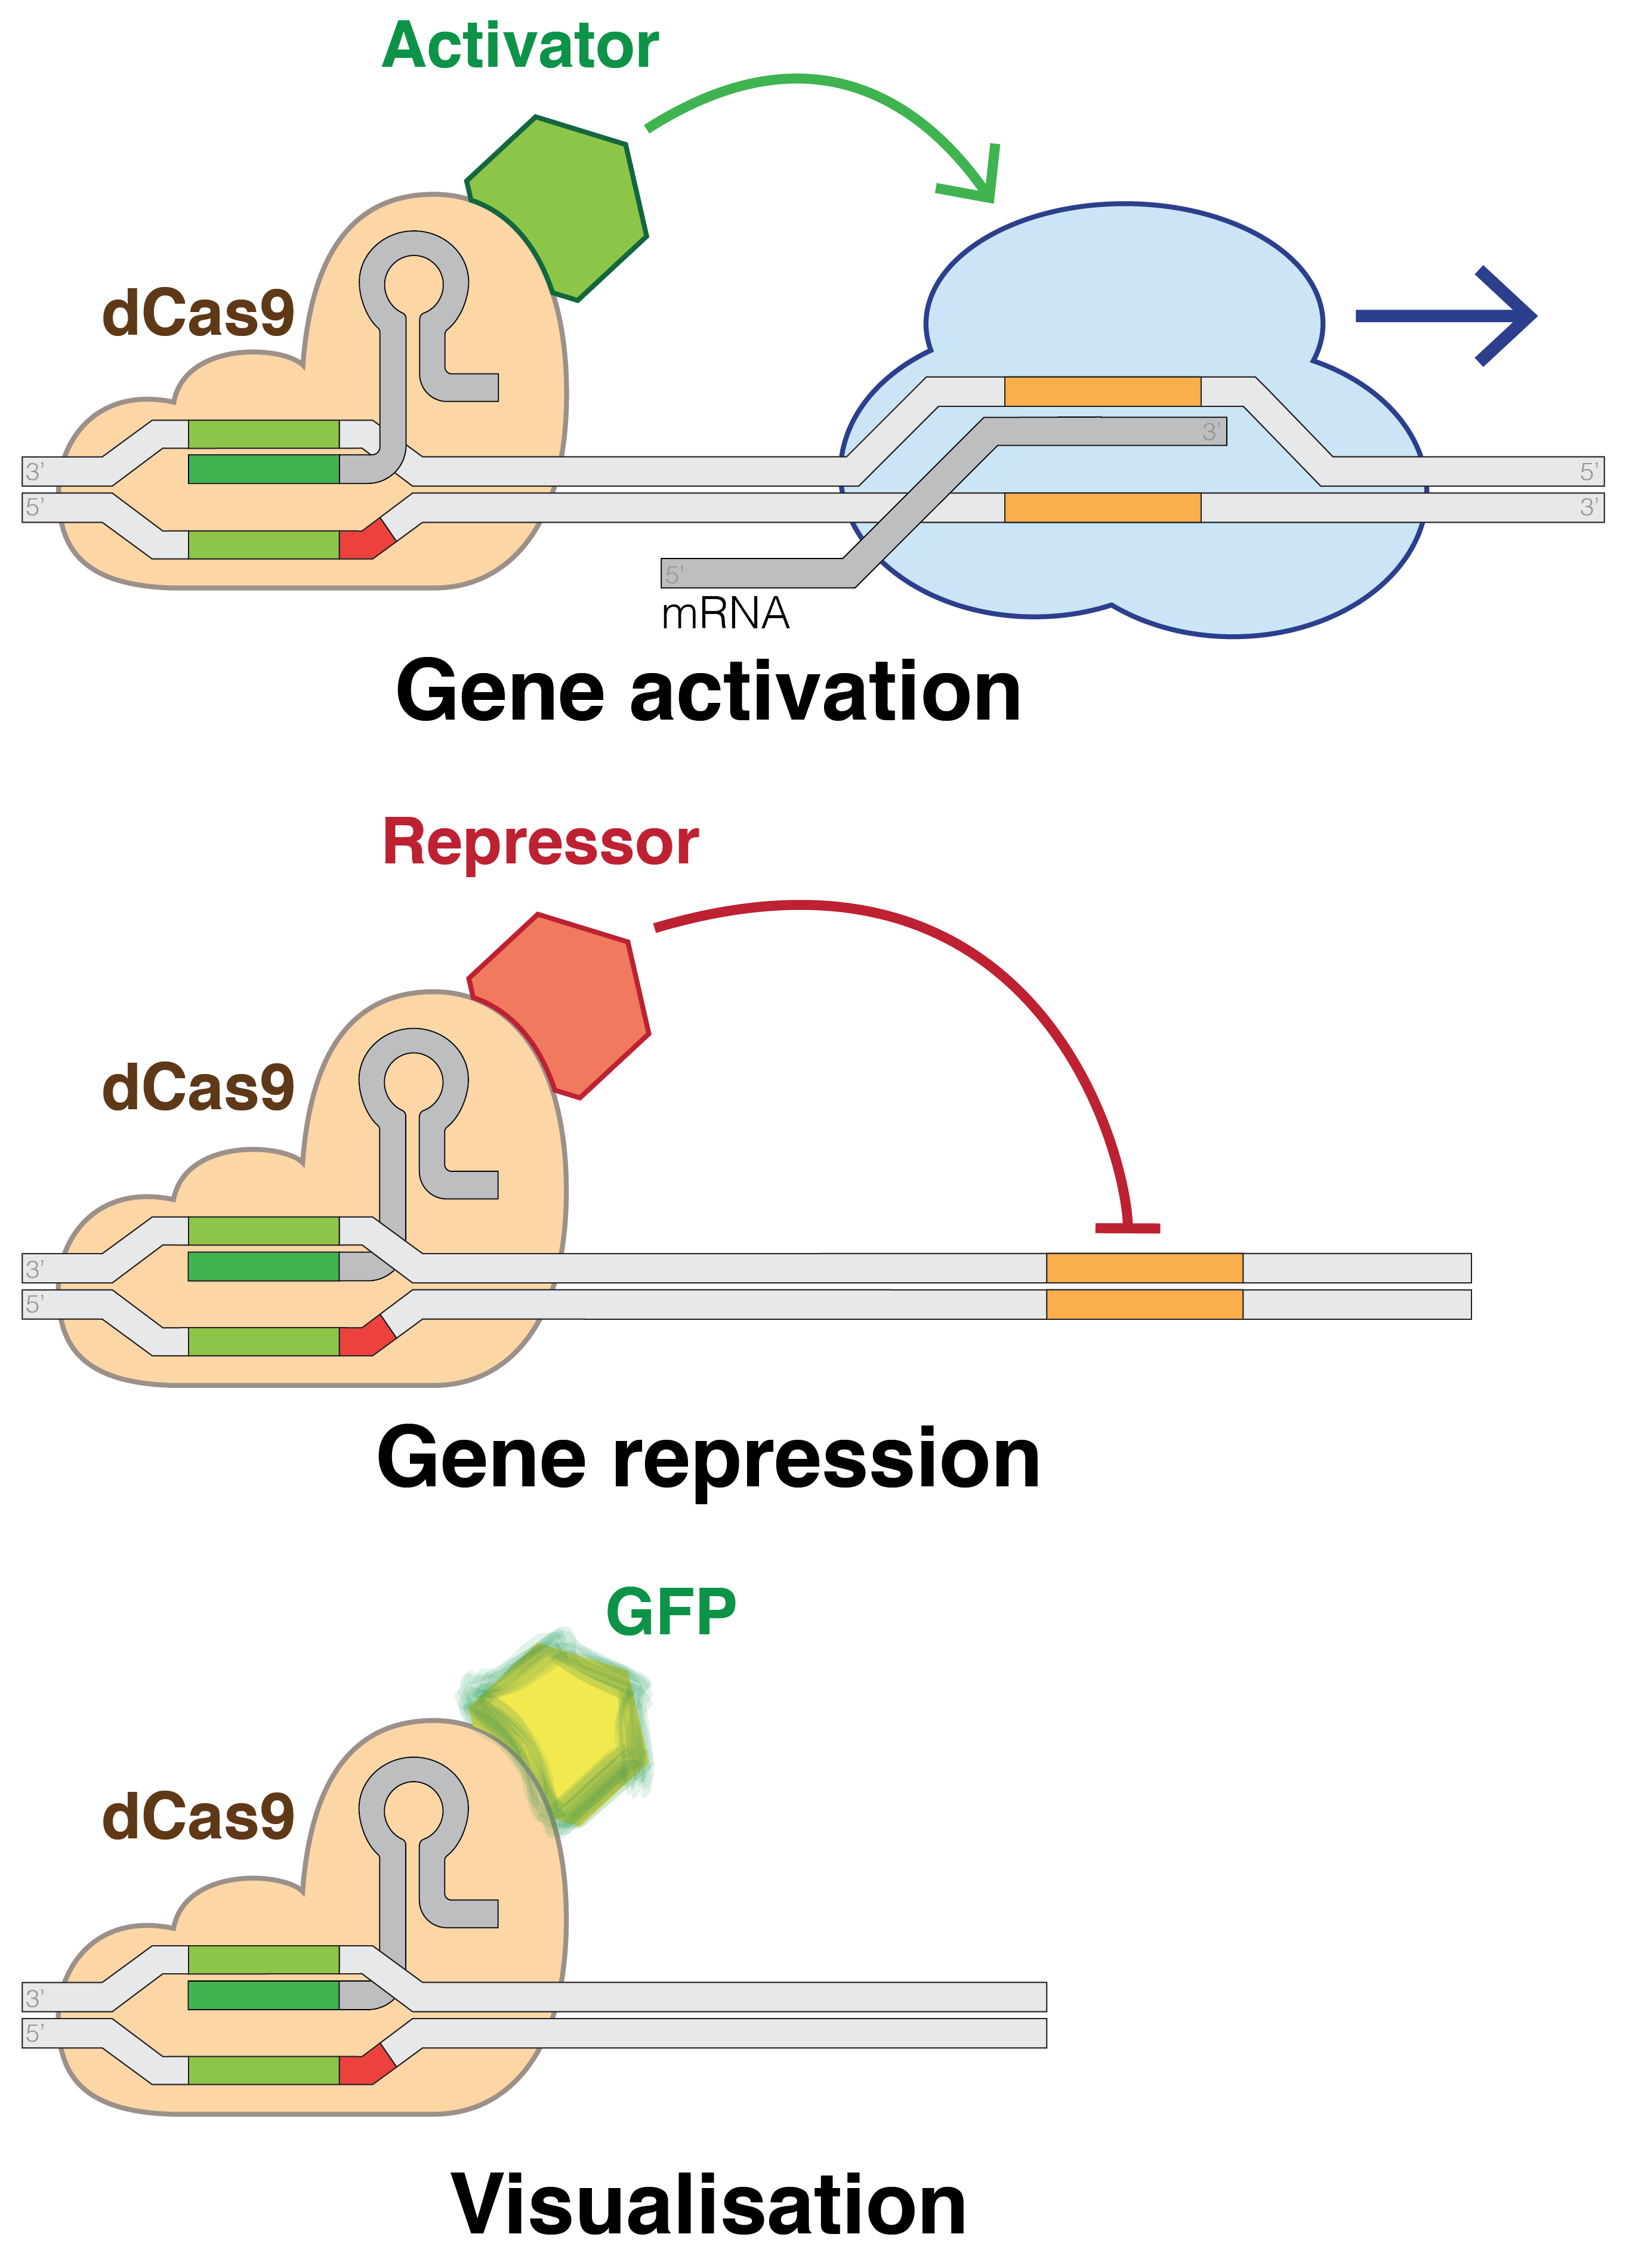
\includegraphics[width=0.4\textwidth]{images/Dead-Cas9_potential_applications.png}\\[.2in]
\caption{dCas9 Potential Application}
\label{dCas9}
\end{figure}
\section{Polymerase Chain Reaction (PCR)}
PCR can \udl{amplify} a single DNA template molecule into $10^9$ copies in a few hours (30 doublings).\\[.2in]
Recall that DNA polymerases extend a 3'-OH in the 5' to 3' direction. The 3'-OH can be on a synthetic DNA primer. DNA base pairing and thus primer annealing is \udl{temperature dependent}.\\[.2in]
PCR creates billions of copies of a region of interest. The region of interest is \udl{defined by synthetic DNA primers}.
\subsection{Reaction Mix and Reaction}
\bd{Reaction mix}
\begin{itemize}
    \item DNA template
    \item Primers complementary to the ends of the target region
    \item dNTPs (i.e. dATP, dCTP, dGTP, dTTP)
    \item Buffer, salts to keep the polymerase happy
    \item Thermotolerant DNA polymerase (e.g. Taq, phusion etc)
\end{itemize}
\bd{Reaction}\\[.1in]
\udl{Thermocycler} is programmed to cycle the temperature
\subsection{Engineering with PCR}
Engineering with restriction enzymes can be hard, where PCR can make things easier.\\[.2in]
Advantages:
\begin{itemize}
    \item Can isolate fragments independently of restriction sites
    \item Can fuse fragments independently of restriction sites
\end{itemize}
Limitations:
\begin{itemize}
    \item length of target region
    \item error rate of DNA polymerase
    \item high \%GC regions
\end{itemize}
\subsection{Seamless joining of DNA fragments with PCR}
\begin{enumerate}
    \item PCR - amplifying left fragment
    \begin{figure}[h]
    \centering
    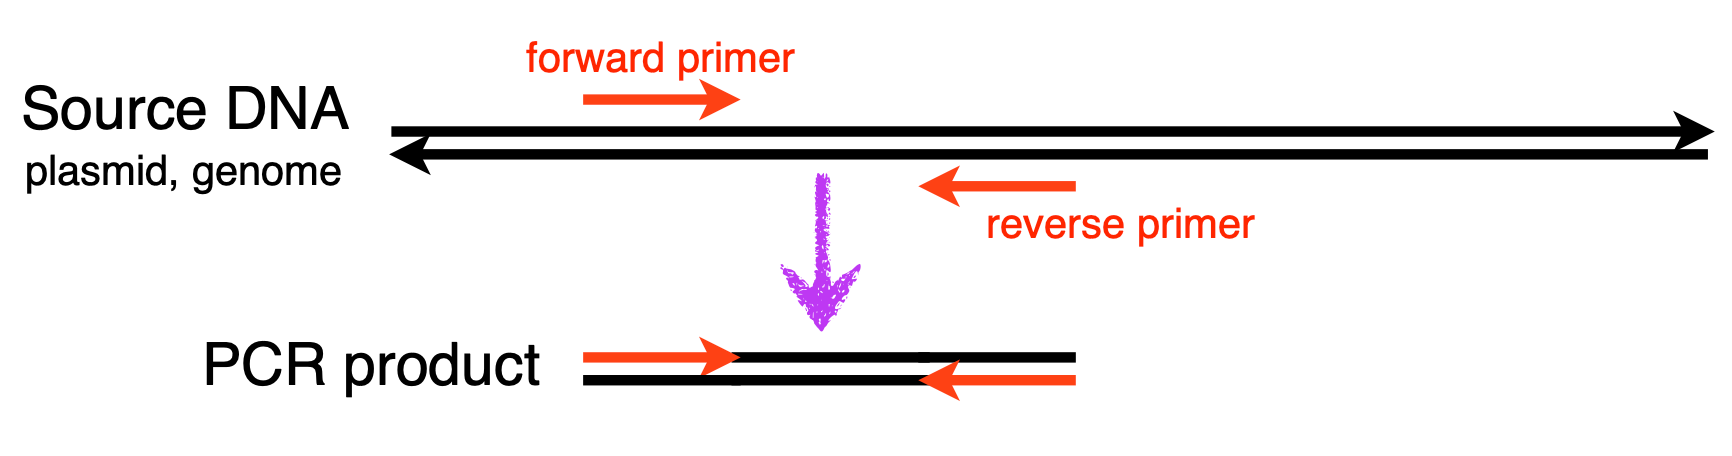
\includegraphics[width=0.6\textwidth]{images/4-3-1.png}\\[.2in]
    \caption{Step 1 - PCR amplifying left fragment}
    \end{figure}
    \item PCR - amplifying right fragment: N.B. \udl{forward primer} contains \udl{same sequence} as end of Step 1 PCR product.
    \begin{figure}[h]
    \centering
    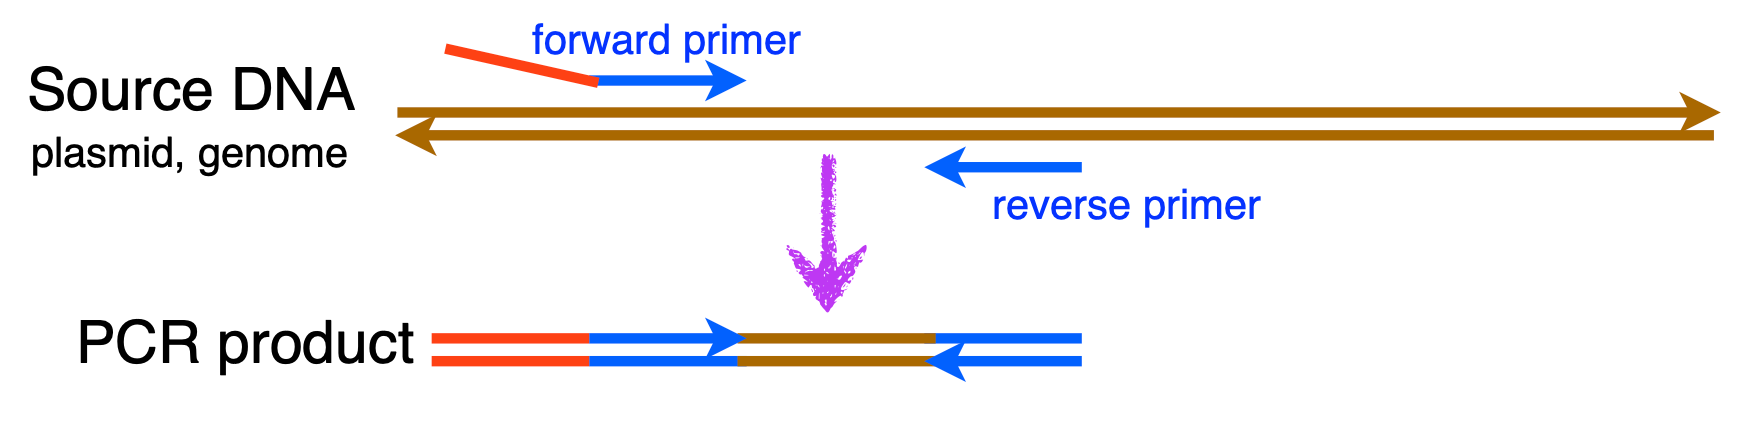
\includegraphics[width=0.6\textwidth]{images/4-3-2.png}\\[.2in]
    \caption{Step 2 - PCR simplifying right fragment}
    \end{figure}
    \item PCR reaction using products from steps 1 + 2 mixed together
    \begin{figure}[h]
    \centering
    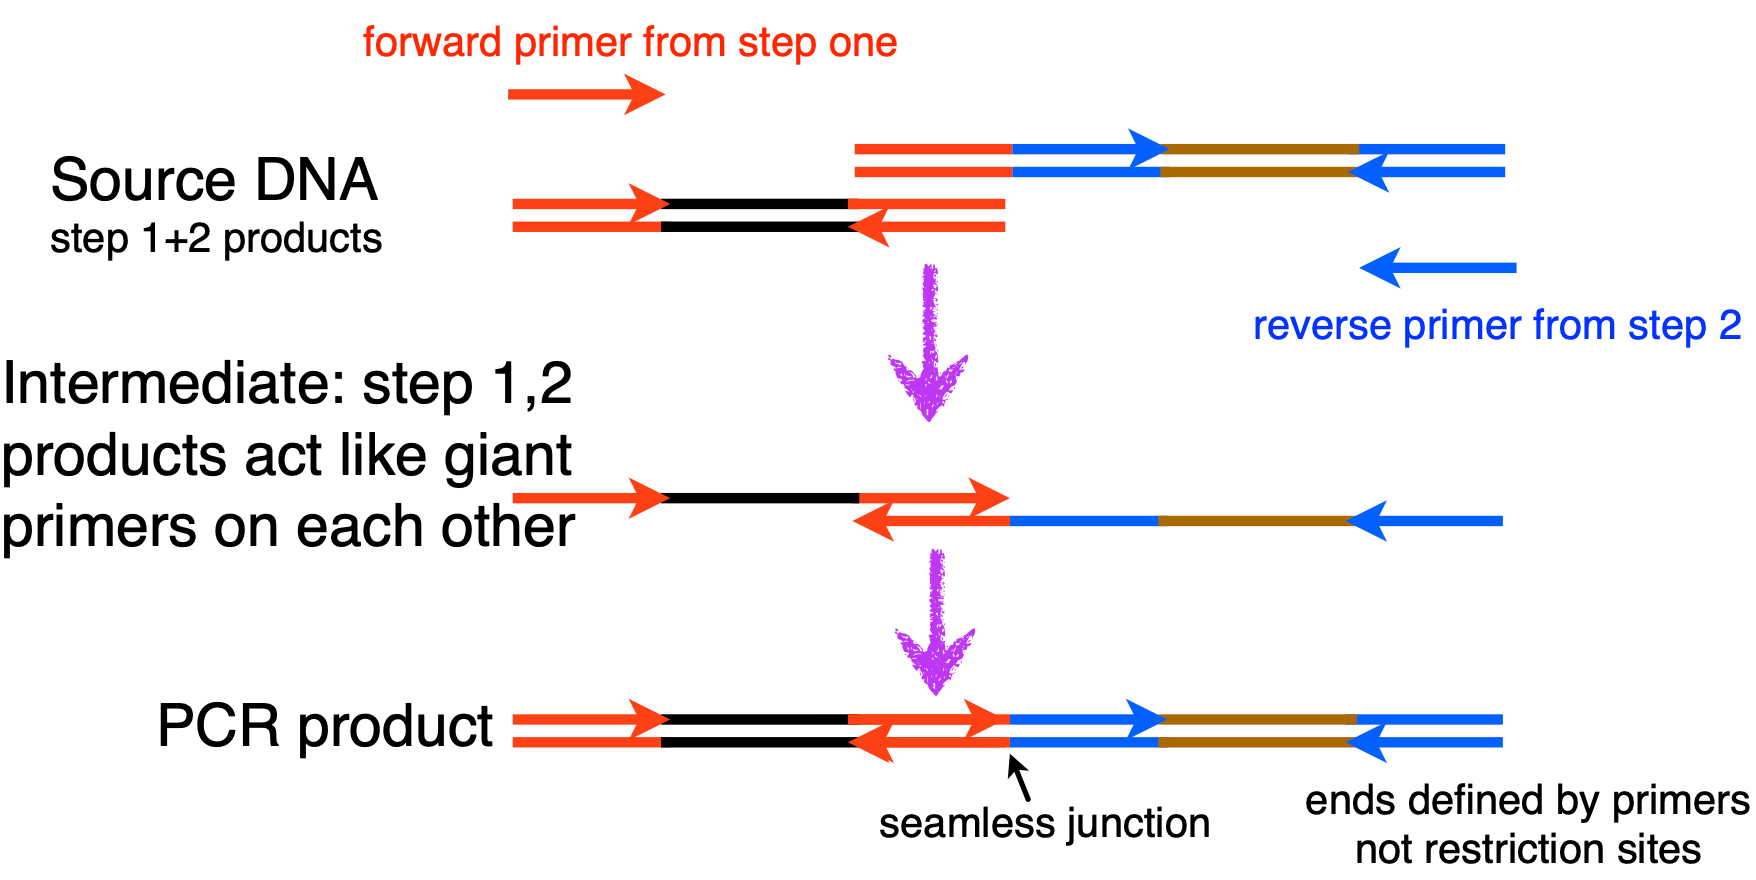
\includegraphics[width=0.6\textwidth]{images/4-3-3.png}\\[.2in]
    \caption{Step 3 - PCR reaction using products from step 1 and 2}
    \end{figure}
\end{enumerate}
\subsection{Things that can go wrong with PCR}
Assume fresh and correct buffers and enzymes and that thermocycler is programmed correctly.
\begin{itemize}
    \item No product: check primer design, decrease annealing temperature, vary MgCl\textsubscript{2} levels.
    \item Multiple products: check primer design, use hot start enzyme, increase annealing temperature, vary MgCl\textsubscript{2} levels.
    \item Product in negative control: contamination (use laminar air flow hood, filter tips).
    \item Primer dimers\footnote{primers self-prime or prime on each other}: redesign primers.
\end{itemize}

\section{Gibson Assembly}
Limitations:
\begin{itemize}
    \item Few. Cost for 100,0000 base scale synthesis
    \item T5 exonuclease will destroy small fragments
\end{itemize}
Advantage:
\begin{itemize}
    \item seamless joining of arbitrary DNA fragments
    \item multiple fragments can be joined in one step
    \item currently cheaper than de novo synthesis
\end{itemize}

\section{De novo synthesis}
Advantage:
\begin{itemize}
    \item independent of restriction enzymes
    \item independent of ability to PCR fragment of interest
    \item allows complete resign of DNA sequence
\end{itemize}
Limitations:
\begin{itemize}
    \item cost (but dropping rapidly)
    \item Scale: ~1kb fragments are ordered by many labs
\end{itemize}
N.B. Small scale sythesis of ~20-50nt DNA oligonucleotides\footnote{a polynucleotide whose molecules contain a relatively small number of nucleotides.} underpins PCR (the primers), DNA sequencing (the primer). 
\chapter{Case study}

\section{Codon optimisation}
Recall the redundant mapping from codons to amino acid and the basic structure of a bacterial gene. In prokaryotes functionally related genes are often grouped in operons\footnote{a unit made up of linked genes which is thought to regulate other genes responsible for protein synthesis.}.
\subsection{Introduction to codon optimisation}
The amino acid code is redundant. Different organisms have different preferences for particular codons. The selection pressure is primarily on growth rate. It is the efficiency optimisation that the organism has done doing evolution. For example, match the codon usage of the gene construct and the host organism; Use the codons found in highly expressed genes.
\subsection{Which are the best codons to use}
A research by ATUM suggested that Genes differing only in synonymous codon usage expressed protein at levels ranging from undetectable to 30\% of cellular protein. It is not those codons most abundant in highly expressed \textit{E. coli} proteins that are the best codons to use, instead, it is the codons read by tRNAs that are \udl{most highly charged} under conditions of amino acid starvation.

\section{Recombinant Insulin}
\subsection{Introduction to Genetic Engineering}
Broadly, genertic engineering is the directed modification of an organism's genetic makeup.\\[.1in]
\udl{Recombinant protein expression} is the process of expressing non-native proteins in an organism. Treat the organism as molecular machine, into which specific DNA sequences are introduced. Introduce DNA with non-native genes, from which the cell will produce a non-native protein (aka \udl{heterologous} or \udl{recombinant protein})
\begin{enumerate}[itemsep=0mm]
    \item to produce a valuable protein product
    \item to create an organism with favourable properties.
\end{enumerate}
\subsection{Genetic Parts and Tools}
To enable recombinant protein expression, we need to create a functional gene.
\begin{figure}[h]
\centering
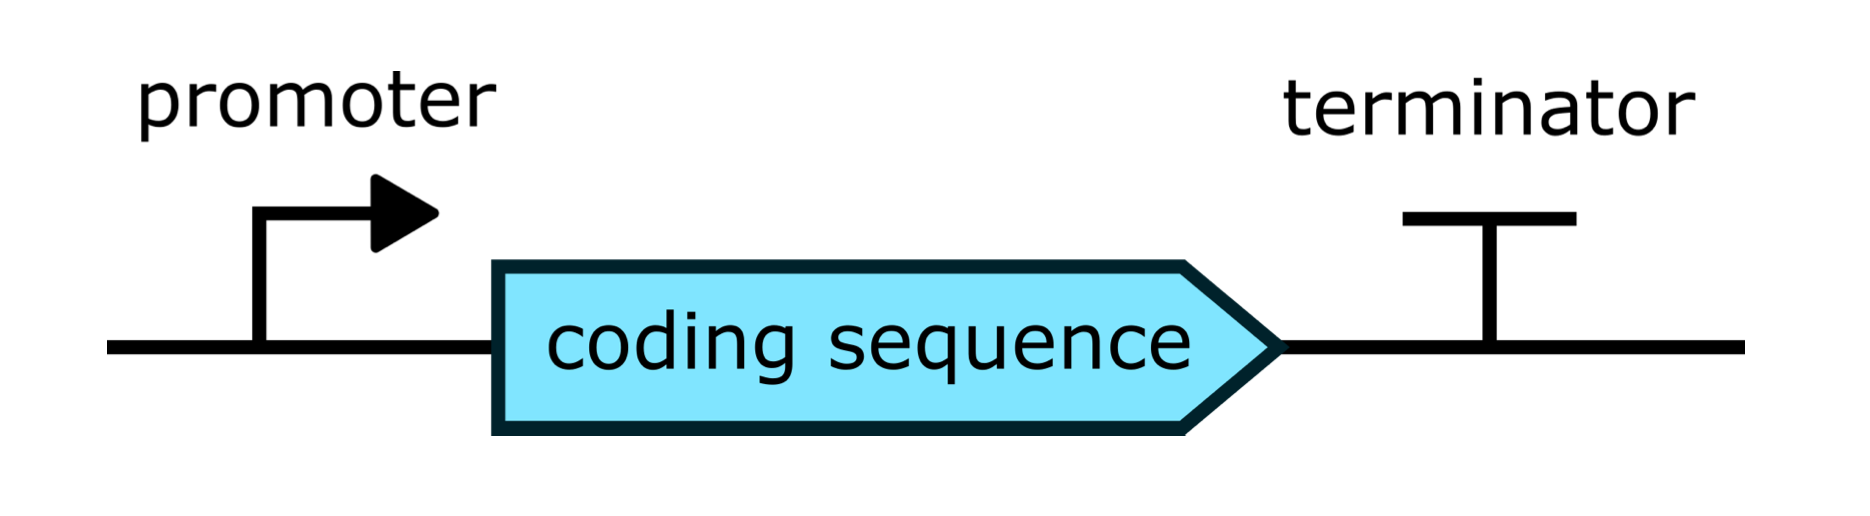
\includegraphics[width=0.8\textwidth]{images/5-1.png}\\[.2in]
\caption{Desirable gene structure}
\end{figure}
\FloatBarrier
\begin{itemize}
    \item Promoters - initiate transcription
    \begin{enumerate}
        \item Can be constitutive or regulated (P\textsubscript{Iac} is IPTG-inducible, P\textsubscript{BAD} is arabinose-inducible)
        \item Regulation enables control of protein expression
        \item Promoters have a range of 'strengths' that determine that levels of protein expressed
    \end{enumerate}
    \item Coding sequences (CDSs) - encode protein amino acid sequence
    \begin{enumerate}
        \item Also known as open reading frames (ORFs)
        \item Functional protein subdomains can be fused together
        \item Short tags direct proteins for specific cellular compartments in Eukaryotes
        \item Affinity tags facilitate the purification of recombinant proteins
    \end{enumerate}
    \item Terminators - stop transcription
\end{itemize}
\subsection{Coding Sequences (CDSs) -- Affinity Tags}
\begin{figure}[h]
\centering
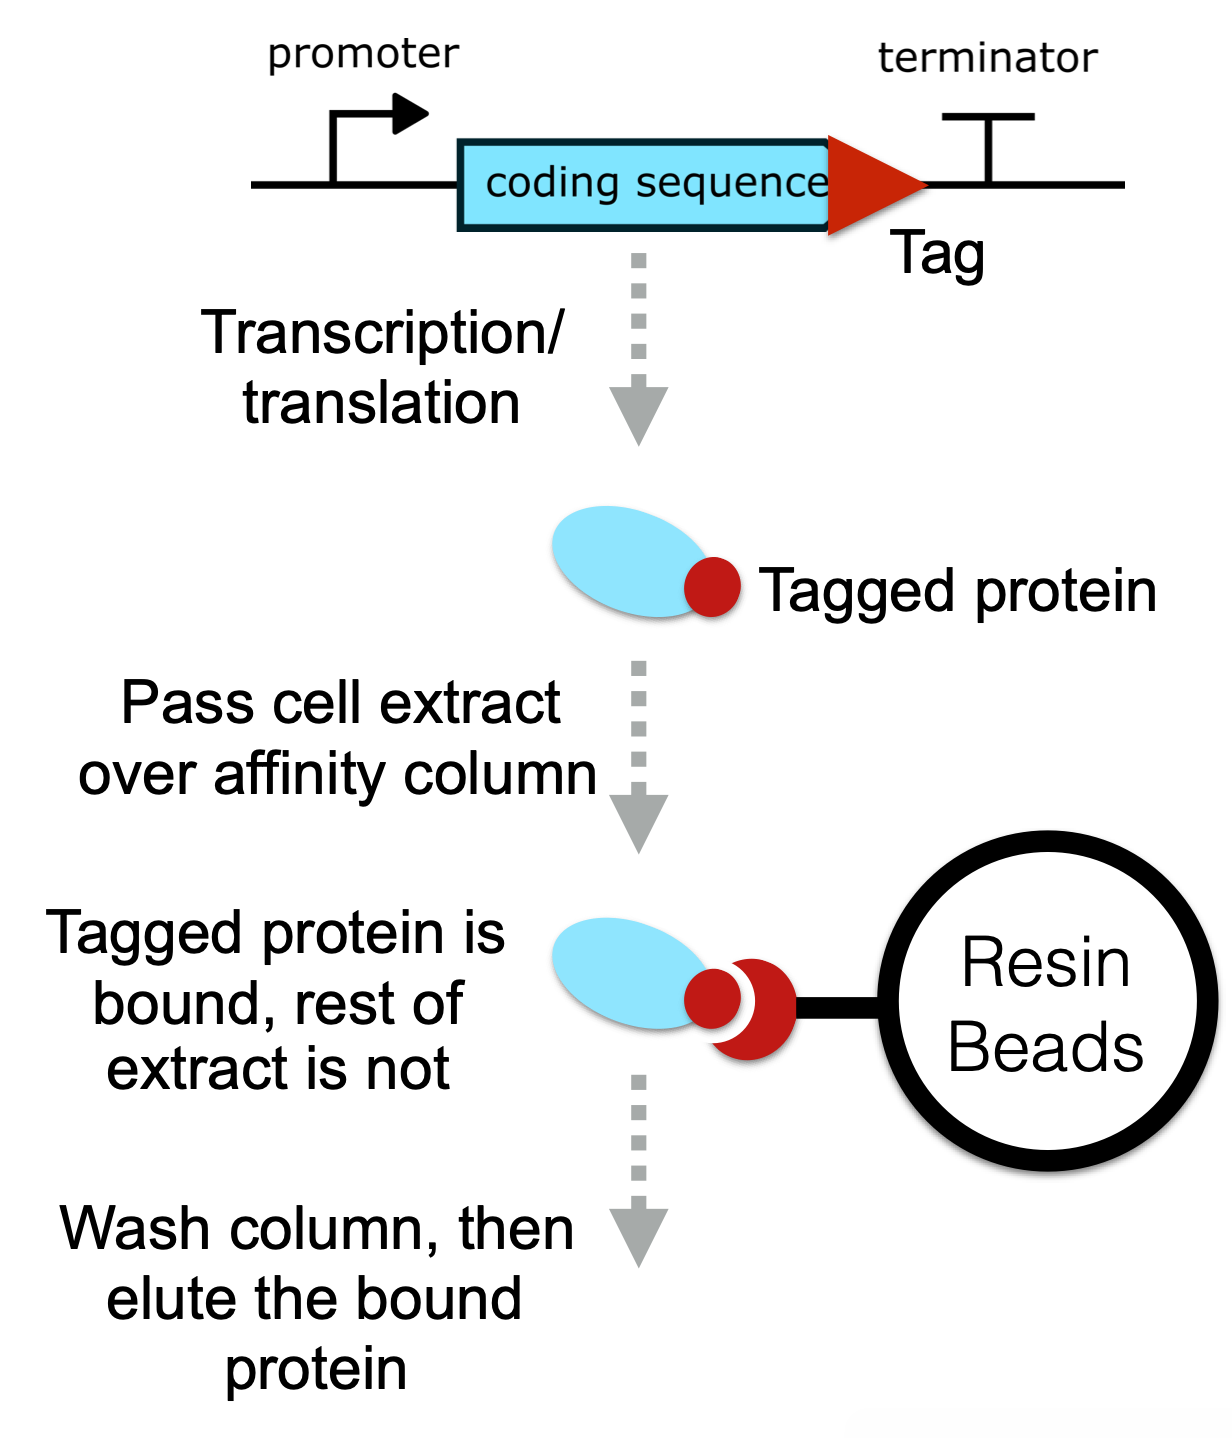
\includegraphics[width=0.5\textwidth]{images/5-2.png}\\[.2in]
\caption{Affinity Tags}
\end{figure}
\FloatBarrier
\begin{itemize}
    \item Affinity tags enable protein purification through interaction with solid phase. 
    \item Most often at N-terminus or C-terminus.
    \item e.g. 6x histidine tag binds Ni\textsuperscript{2+} ions immobilised\footnote{prevent (something or someone) from moving or operating as normal} on agarose resin. 
    \item 3xFLAG tag has enterokinase cleavage site allowing elution\footnote{remove (an adsorbed substance) by washing with a solvent} of the tag-free protein.
\end{itemize}
\subsection{Host Organisms}
Different host organisms or 'chassis' have different properties, choosing which to work with is important.\\[.1in]
% Table ---
\begin{table}[h]
\centering
\resizebox{0.9\textwidth}{!}{%
\begin{tabular}{@{}cll@{}}
\toprule
Organism & \multicolumn{1}{c}{Class} & \multicolumn{1}{c}{Properties} \\ \midrule
\textit{E. coli} & \begin{tabular}[c]{@{}l@{}}Gram-negative \\ bacterium\end{tabular} & \begin{tabular}[c]{@{}l@{}}Easy to grow, relatively simple cellular \\ physiology, numerous genetic tools\end{tabular} \\
\begin{tabular}[c]{@{}c@{}}\textit{S. cerevisiae}\\ (budding yeast)\end{tabular} & \begin{tabular}[c]{@{}l@{}}'simple' eukaryote\end{tabular} & \begin{tabular}[c]{@{}l@{}}Easy to grow, efficient protein \\ secretion, complex metabolism\end{tabular} \\
\begin{tabular}[c]{@{}c@{}}Mammalian cells\end{tabular} & \begin{tabular}[c]{@{}l@{}}complex eukaryote\end{tabular} & \begin{tabular}[c]{@{}l@{}}More difficult to grow, an produce \\ true human proteins\end{tabular} \\ \bottomrule
\end{tabular}%
}
\caption{Host organisms}
\label{tab:organisms}
\end{table}
\FloatBarrier
Eukaryotes are capable of various post-translational modifications (e.g. glycosylation, proteolytic processing) and use specific signals to direct proteins to be inserted into the membrane or secreted.
\subsection{Engineering recombinant insulin}
Diabetes mellitus is a common disorder that can be fatal if not treated. Many diabetics require daily injections of a peptide hormone insulin to regulate their blood glucose levels. Pig insulin used to be used to treat diabetics, but production methods were inconsistent and not cost-effective. Insulin was the \udl{first hormone} to be produced by recombinant DNA technology.
\subsection{Recombinant Insulin}
\bd{Design brief}
\begin{itemize}
    \item make recombinant insulin that can be produced in \udl{large volumes}, purified easily, \udl{functional in humans} and \udl{safe}.
    \item Using \textit{E.coli} as host
\end{itemize}
\bd{Issues}
\begin{itemize}
    \item preproprotein is processed into mature protein
    \item cleavage removes N-terminus (no methionine left)
    \item middle is proteolytically removed
    \item mature A and B polypeptides held together with disulfide bonds
\end{itemize}
Today, much of recombinant insulin is produced in the budding yeast. \textit{S.} \textit{cerevisiae}.

\section{Antibodies}
\subsection{Antibody immune response}
Antibodies have a number of effects on their targets. Antibodies form an important part of the \udl{adaptive immune response}.
\begin{enumerate}
    \item \bd{Neutralisation} \\ Antibodies prevent a virus or toxic protein from binding their target.
    \item \bd{Opsonisation} \\ A pathogen tagged by antibodies is consumed by a macrophage or neutrophil.
    \item \bd{Complement activation} \\ Antibodies attached to the surface of a pathigen cell activate the complement system.
\end{enumerate}
Antibodies (Abs) have natural properties that make them high useful:
\begin{itemize}
    \item Abs recognise antigens with exquisite specificity
    \item Abs are highly diverse with known structural properties
    \item Abs are robust molecules that are naturally long lived
    \item Abs are a normal part of the human immune system
    \item Around $10^{10}$ variants in humans
\end{itemize}
\subsection{Antibodies structure}
Antibodies is \udl{Y-shaped}. Proteins are produced by \udl{B cells}. They bind specific targets. They consist of \udl{two heavy and two light chains}. Different antibodies bind different antigens (Ag) based on \udl{variations in the antigen-biding site} (5). It has \udl{two identical Ag binding sites} increases Ab affinity\footnote{the degree to which a substance tends to combine with another.}.
\begin{figure}[h]
\centering
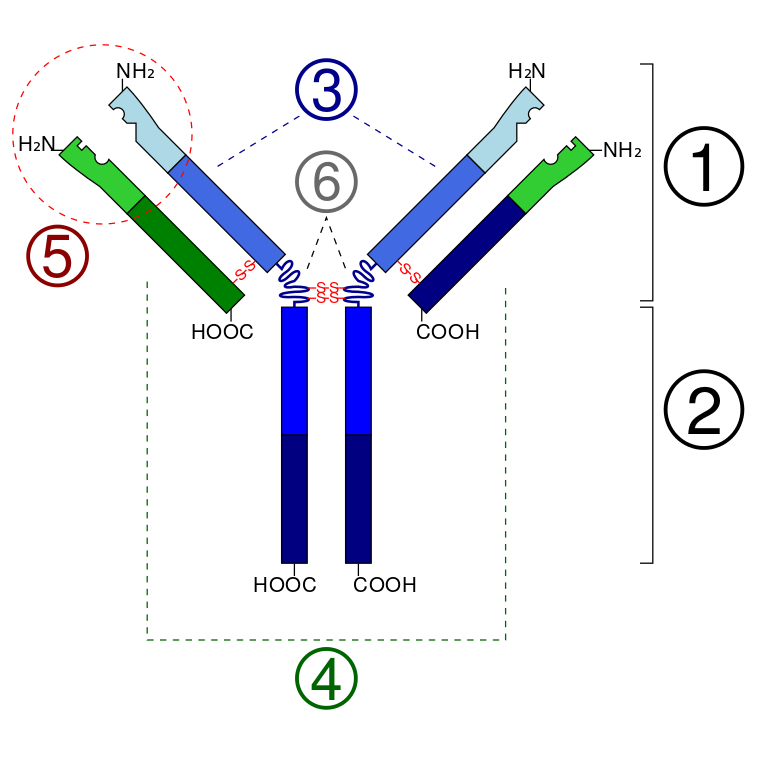
\includegraphics[width=0.6\textwidth]{images/Immunoglobulin_basic_unit.svg.png}\\[.1in]
\caption{Antibody structure}
\end{figure}
\FloatBarrier
\begin{enumerate}[noitemsep]
    \item Fragment antigen binding (Fab) region
    \item Fragment crystallisable (Fc) region
    \item Heavy chain (blue): 1 variable and 3 constant domains
    \item Light chain (green): 1 variable and 1 constant domain
    \item Antigen binding site
    \item Hinge region
\end{enumerate}
The heavy and light chains are composed of subdomains, each with a common beta-sheet rich immunogobulin (Ig) fold. The variable domain at the tip of each Fab arm has \udl{highly variable amino acid sequence}. This variation is what accounts for antigen specificity.
\subsection{Antibodies: Complementary Determining Regions}
The amino acid sequence of the complementarity determining regions (CDRs) aka \udl{hypervariable} regions dictate antigen specificity.
\subsection{Antibodies: gene to protein}
uring B cell maturation, \udl{\textit{somatic recombination}} leads to joining of gene segments at DNA level. Combinatorial diversity results in many possible amino acid sequences \udl{at the CDRs}. Heavy chain: 44x V, 27x D, 6x J segments each with different sequence. Light chain: many V, J segments (no D) -- Totally about \udl{$3\times10^{11}$ possibilities}. Affinity maturation (directed mutation) creates further diversity.
\subsection{Monoclonal Antibodies: Therapeutic uses}
\bd{Scale: Producing Monoclonal Antibodies (mAbs)}
\begin{enumerate}[itemsep=0mm]
    \item Challenge mouse with antigen.
    \item Purify Iymphocytes (B cells, motal, HGPRT+) from spleen.
    \item Fuse with myeloma cells (immortal, HGPRT-).
    \item Select for \udl{hybridoma clones} (fused cells, HGPRT+, immortal).
    \item Screen for antibody production against target antigen.
    \item Positive clones secrete \udl{monoclonal antibodies} into the culture medium and can be grown indefinitely.
\end{enumerate}
\bd{Antibodies as therapeutics}
\begin{itemize}
    \item Monoclonal antibodies (mAb) recognise one epitope (shape) with very high specificity
    \item Mediate immune responses to pathogens
    \item Can interfere with cancer cell function or autoimmune conditions
    \item Can conjugate drugs and radioactive atoms to antibodies and deliver them to specific tissues and cells
\end{itemize}
Antibodies are developed by immunising mice and other animals. If used in humans these antibodies are themselves recognised as \udl{foreign} and attacked by the human immune system.

\section{Engineering Antibodies}
\subsection{Engineering antibodies for use in human}
Solutions to problem of animal antibodies being antigenic in humans.
\begin{itemize}
    \item Chimaeric Ab: transplant mouse VL/VH sequence to human Ab.
    \item Humanised Ab: transplant mouse CDR loop sequence to human Ab.
\end{itemize}
\subsection{Humanising antibodies}
\bd{Jargons}
\begin{itemize}[noitemsep]
    \item Mouse -omab 
    \item Chimaeric -ximab 
    \item Humanised -zumab 
    \item Human -mumab
\end{itemize}
\bd{Identifying and modifying CDRs}\\[.1in]
Aligning protein sequences allows visualisation of the variable and constant regions in antibodies from each organism.\\[.2in]
\bd{Alternative methods for generating mAbs}\\[.1in]
Genetically engineer mice to carry human antibody genes.\\[.2in]
\bd{Phage display}: engineer the human antibody repertoire into the surface of bacteriophage and then select for phage that bind to antigen. The variable regions of light and heavy chains are fused and expressed on the surface of a bacteriophage. The library is bound to antigen and non/weak-binders washed off. Tightly bound phage are eluted and clones are generated by infection of E. coli then sequenced. This is also known as \udl{\textit{panning}}.
\subsection{Insudtrial scale mAb production}
Engineer mammalian cells to produce human antibodies e.g. Chinese hamster ovary (CHO) cells. Mammalian cells, so possess PTM machinery for disulphide bonds and glycosylation. Cells grown in industrial bioreactors. More than 10,000 L scale production systems. There is a large and growing market for mAbs. Growing numbers of mAb are being approved for clinical use, currently about 100 (US FDA).
\subsection{Summary}
\begin{itemize}
    \item Recombinant human insulin and mAb therapies are great examples of genetic engineering and its utility.
    \item Recombinant protein expression let’s you produce naturally-occurring proteins efficiently.
    \item Produce entirely new-to-nature proteins with useful properties.
    \item Debates over the ethics of genetic engineering are very important, these case studies exemplify the societal benefits this technology can bring.
\end{itemize}

 

\bibliography{Sample}

\end{document}
